\documentclass[dvipdfmx,10pt,journal,compsoc]{IEEEtran}

\usepackage[ruled, vlined]{algorithm2e}    % \begin{algorithm2e}
\usepackage{amsmath}        % \begin{align*}
\usepackage{amssymb}        % \mathbb{A}
\usepackage{amsthm}         % \newtheorem
\usepackage{bm,bbm}         % \bm{A}, \bbm{1}
\usepackage{booktabs}       % \toprule, \midrule, \bottomrule
\usepackage{subcaption}        % \captionsetup
\usepackage{enumitem}       % \begin{enumerate}[label=(\alph*)]
\usepackage{hyperref}       % \href{URL}{text}
\usepackage{ifthen}         % \ifthenelse
\usepackage{lipsum}         % \lipsum
\usepackage{mathrsfs}       % \mathscr{A}
\usepackage{mathtools}      % \mathrlap
\usepackage{optidef}        % \begin{mini*}{x}{f(x)}{}{}
\usepackage{orcidlink}      % \orcidlink
\usepackage{physics}        % \qty, \norm, \abs
\usepackage{subfiles}       % \subfile{file}
\usepackage{thm-restate}    % \begin{restatable}{theorem}{thm}
\usepackage{tikz}           % \begin{tikzpicture}
\usepackage{xparse}         % \NewDocumentCommand
% \usepackage{calc}         % \setlength
% \usepackage{cancel}       % \cancel
% \usepackage{parskip}      % \setlength{\parskip}{0.5em}
% \usepackage{csvsimple}    % \csvautotabular
% \usepackage{diagbox}      % \diagbox
% \usepackage{dsfont}       % \mathds{1}
% \usepackage{epsfig}       % \epsfig
% \usepackage{fancybx}      % \ovalbox
% \usepackage{float}        % \begin{figure}[H]
% \usepackage{lipsum}       % \lipsum
% \usepackage{listings}     % \begin{lstlisting}
\usepackage{makecell}     % \makecell{L1\L2}
% \usepackage{multicol}     % \begin{multicols}{2}
% \usepackage{multirow}     % \multirow
% \usepackage{nicematrix}   % \begin{NiceMatrix}
% \usepackage{qcircuit}     % \Qcircuit
% \usepackage{siunitx}      % \SI{1}{\second}
% \usepackage{stfloats}     % \begin{figure*}
% \usepackage{subcaption}   % \begin{subfigure}
% \usepackage{ulem}         % \sout
% \usepackage{wrapfig}      % \begin{wrapfigure}
% \usepackage[all]{xy}      % \xymatrix
% \usepackage[dvipdfmx]{graphicx}
% \usepackage[square, sort, comma, numbers]{natbib}

\hypersetup{colorlinks=true,linkcolor=blue,citecolor=blue,urlcolor=blue}

\definecolor{cA}{HTML}{0072BD}
\definecolor{cB}{HTML}{EDB120}
\definecolor{cC}{HTML}{77AC30}
\definecolor{cD}{HTML}{D95319}

\newcommand{\red}[1]{\textcolor{red}{#1}}
\newcommand{\blue}[1]{\textcolor{blue}{#1}}
\newcommand{\cyan}[1]{\textcolor{cyan}{#1}}
\newcommand{\gray}[1]{\textcolor{gray}{#1}}
\newcommand{\green}[1]{\textcolor{green}{#1}}
\newcommand{\brown}[1]{\textcolor{brown}{#1}}
\newcommand{\black}[1]{\textcolor{black}{#1}}
\newcommand{\orange}[1]{\textcolor{orange}{#1}}
\newcommand{\st}{\text{ s.t. }}
\newcommand{\Img}[1]{\mathrm{Im}\qty(#1)}
\newcommand{\Ker}[1]{\mathrm{Ker}\qty(#1)}
\newcommand{\Supp}[1]{\mathrm{supp}\qty(#1)}
\newcommand{\Rank}[1]{\mathrm{rank}\qty(#1)}
\newcommand{\floor}[1]{\left\lfloor #1 \right\rfloor}
\newcommand{\ceil}[1]{\left\lceil #1 \right\rceil}
% C++ (https://tex.stackexchange.com/questions/4302/prettiest-way-to-typeset-c-cplusplus)
\newcommand{\Cpp}{C\nolinebreak[4]\hspace{-.05em}\raisebox{.4ex}{\relsize{-3}{\textbf{++}}}}
% https://tex.stackexchange.com/questions/28836/typesetting-the-define-equals-symbol
\newcommand{\defeq}{\coloneqq}
\newcommand{\eqdef}{\eqqcolon}
% https://tex.stackexchange.com/questions/5502/how-to-get-a-mid-binary-relation-that-grows
\newcommand{\relmiddle}[1]{\mathrel{}\middle#1\mathrel{}}

% https://tex.stackexchange.com/questions/564216/newcommand-for-each-letter
\ExplSyntaxOn
\NewDocumentCommand{\definealphabet}{mmmm}{
\int_step_inline:nnn{`#3}{`#4}{
\cs_new_protected:cpx{#1 \char_generate:nn{##1}{11}}{
\exp_not:N #2{\char_generate:nn{##1}{11}}}}}
\ExplSyntaxOff

\definealphabet{bb}{\mathbb}{A}{Z}
\definealphabet{rm}{\mathrm}{A}{Z}
\definealphabet{cal}{\mathcal}{A}{Z}
\definealphabet{frak}{\mathfrak}{a}{z}
% \definealphabet{scr}{\mathscr}{A}{Z}
% \definealphabet{frak}{\mathfrak}{A}{Z}

\newtheorem{theorem}{Theorem}
\newtheorem{proposition}{Proposition}
\newtheorem{lemma}{Lemma}
\newtheorem{definition}{Definition}
\newtheorem{corollary}{Corollary}
\newtheorem{remark}{Remark}
\newtheorem{example}{Example}
\newtheorem{assumption}{Assumption}

% https://qiita.com/rityo_masu/items/efd44bc8f9229e014237
\allowdisplaybreaks[4]

\usetikzlibrary{
  3d,
  % fit,
  calc,
  math,
  matrix,
  patterns,
  backgrounds,
  arrows.meta,
  shapes.geometric,
  decorations.pathmorphing,
}

% \providecommand{\main}{.}
\newboolean{isMain}
\setboolean{isMain}{true}

\begin{document}
\bstctlcite{IEEEexample:BSTcontrol}

\title{
  An Initial Placement
  for Fruchterman--Reingold force model
  with Coordinate Newton Direction
}
\author{
  Hiroki Hamaguchi\,\orcidlink{0009-0005-7348-1356}
  Naoki Marumo\,\orcidlink{0000-0002-7372-4275}
  Akiko Takeda\,\orcidlink{0000-0002-8846-4496}
  % <-this % stops a space
}

\IEEEtitleabstractindextext{%
  \begin{abstract}
    Graph drawing is a fundamental task in information visualization, with the Fruchterman--Reingold (FR) force model being one of the most popular choices.
    This layout can be interpreted as a solution of a continuous optimization problem, which can be solved using the FR algorithm, a gradient descent-like method, or the L-BFGS algorithm, quasi-Newton method.
    However, these methods are computationally expensive per iteration, which makes achieving high-quality visualizations for large-scale graphs challenging.

    In this paper, to accelerate the optimization process, we propose a new initial placement with coordinate Newton direction.
    We first reformulate the problem as a discrete optimization problem using a hexagonal lattice, and then iteratively move a randomly selected vertex along the coordinate Newton direction.
    We can use the FR algorithm or L-BFGS algorithm to obtain the final placement.

    We demonstrate the effectiveness of our proposed approach through experiments, highlighting the potential of coordinate block based methods for graph drawing tasks.
    Additionally, we suggest combining our method with other graph drawing techniques for further improvement.
    We hope that this work will inspire future research of coordinate block based methods not only in graph drawing but also in broader graph-related applications.
  \end{abstract}
  \begin{IEEEkeywords}
    Graph Drawing,
    Optimization,
    Fruchterman--Reingold Algorithm,
    L-BFGS algorithm
  \end{IEEEkeywords}}
\maketitle


\section{Introduction}\label{sec:introduction}

\IEEEPARstart{G}{raph} is a mathematical structure representing pairwise relationships between objects, and graph drawing is a fundamental tasks in information visualization.
Indeed, numerous kinds of models and algorithms have been proposed~\cite{tutteHowDrawGraph1963,chrobakLineartimeAlgorithmDrawing1995,sugiyamaMethodsVisualUnderstanding1981}, and among these, one of the most popular choices is the force-directed graph drawing.

In force-directed graph drawing, we model a graph as a system of particles with forces acting between them. By simulating the system and seeking the equilibrium of the forces, we can obtain a visualization of the graph.
Among the various force models~\cite{eades1984heuristic,kamadaAlgorithmDrawingGeneral1989}, the Fruchterman--Reingold (FR) force model~\cite{fruchtermanGraphDrawingForcedirected1991,kobourovSpringEmbeddersForce2012} is the central focus of our study.

FR algorithm is the original algorithm for this force model, and it can be regarded as a variant of gradient descent method for the energy function of the model.
FR algorithm is implemented in many modern graph drawing libraries such as NetworkX~\cite{hagberg2008exploring}, Graphviz~\cite{ellsonGraphvizOpenSource2002}, and igraph~\cite{csardiIgraphSoftwarePackage2006}.

However, the FR algorithm has several issues that makes it challenging to achieve high-quality visualizations for large-scale graphs.
First, it suffers from high computational complexity, $\order{n^2}$ per iteration as it is with $n$ being the number of vertices.
Secondly, the occurrence of ``twist''~\cite{cheongSnapshotVisualizationComplex2018} is crucial for the force model, as it can significantly impact the simulation efficiency.
We refer to ``twist'' as unnecessary intersections of edges or tangled structures in visual representations, as shown in the upper half of Fig.~\ref{fig:fig1}.
When ``twist'' exists, mutual interactions may weaken or diminish the forces, causing the simulation process to stagnate.

\begin{figure}[t]
  \centering
  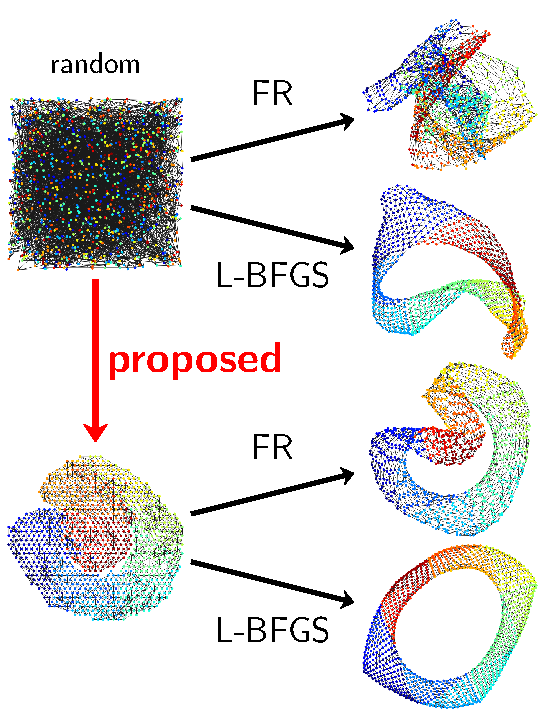
\includegraphics[width=0.8\columnwidth]{fig1/fig1.pdf}
  \caption{
    Comparison of the algorithms for the \texttt{jagmesh1}.
  }
  \label{fig:fig1}
\end{figure}

Approximating or simplifying the model itself is one of the strategies to address these issues in general.
The $n$-body simulation using multipole expansions~\cite{greengardFastAlgorithmParticle1987} or the Barnes--Hut approximation~\cite{barnesHierarchicalLogForcecalculation1986}, gradually refining the layouts using a multilevel approach~\cite{Hu2006EfficientHF} and employing stress majorization~\cite{gansnerGraphDrawingStress2005} are examples of such approaches.

Another strategy is to directly accelerate the simulation process with the forces, in other words, the optimization process of the energy function.
This aligns with the aim of our work.
Recent researches have accelerated the process through various ways, such as adapting to GPU parallel architectures~\cite{gajdosParallelFruchtermanReingold2016}, or utilizing numerical optimization methods.
L-BFGS, a family of quasi-Newton methods, is one of the such methods, and is reported to be effective for graph drawing~\cite{6183577}.
However, since this method just treats the problem as a general optimization problem, there is room for improvement.
Simulated Annealing (SA) is also effective when used as a pre-processing step~\cite{ghassemitoosiSimulatedAnnealingPreProcessing2016}, since SA can deal ``twist'' issues and leads a better visualization combined with the FR algorithm.
However, this work only uses a circle initial placement for unweighted graphs, and the effectiveness of large-scale graphs is unclear since it just repeats to try swapping the positions of two randomly selected vertices.

Based on such advances, in this paper, we propose a new initial placement for the FR force model as depicted in Fig.~\ref{fig:fig1}.
Our goal is to accelerate the optimization process by leveraging the inherent structure of the problem, which has ignored in the L-BFGS algorithm.
To achieve this, we optimize the position of vertices one by one with the Newton direction, which is defined in the coordinate block $\bbR^2$ in the entire variable space $\bbR^{2 \times n}$.
The result provides an initial placement with fewer ``twists'', accelerating the overall optimization process. Our work extends the applicability of initial placement idea to wider range of graphs.
We also demonstrate its effectiveness through various experiments.

The rest of this paper is organized as follows.
In Sec.~\ref{sec:preliminary}, we define the optimization problem we consider and introduce the conventional approaches.
In Sec.~\ref{sec:algorithm}, we propose a new initial placement algorithm.
In Sec.~\ref{sec:experiment}, we show the experimental results.
In Sec.~\ref{sec:challenges}, we discuss the potential of the coordinate based methods, the key concept of our research.
Finally, we discuss future work and conclude the paper in Sec.~\ref{sec:discussion}.

\section{Preliminary}\label{sec:preliminary}

In this section, we formulate the simulation process of the force model as a continuous optimization problem and introduce the conventional approaches to this problem, namely the FR algorithm and the L-BFGS algorithm. We also briefly review the pre-processing step by Ref.~\cite{ghassemitoosiSimulatedAnnealingPreProcessing2016}.

\subsection{Formulation of the Force Model}\label{ssec:forceModel}

Let $\bbR_{> 0} \defeq \qty{ x \in \bbR \mid x > 0 }, \quad \bbR_{\geq 0} \defeq \qty{ x \in \bbR \mid x \geq 0 }$, and let $W = (w_{i,j}) \in \bbR_{\geq 0}^{n \times n}$ be an adjacency matrix of a graph $G_W = (V, E)$, where $V = \qty{v_i \mid 1 \leq i \leq n}$ is a set of vertices and $E = \qty{\{v_i, v_j\} \mid w_{i,j} > 0}$ is a set of edges.
For simplicity, we sometimes identify each vertex $v_i$ with its index $i$, and use notation such as $(i, j) \in E$.
We call $w_{i,j}$ as a weight of the edge $\{v_i,v_j\}$.

We will only consider undirected connected graphs with non-negative weights.
Although the FR algorithm in NetworkX, for example, can handle directed unconnected graphs with negative weights, this paper does not focus on such cases.
For directed graphs, slight modifications of algorithms or converting graphs to undirected ones may be effective.
For unconnected graphs, algorithms can be applied to each connected component independently.
When negative weights are present, the optimization Prob.~\eqref{eq:fr} defined below can be unbounded, but with non-negative weights and the connectivity of $G$, the problem is always bounded and solvable.
In summary, the conditions for $W$ is formulated as follows:
\begin{equation}\label{eq:WCondition}
  W \in \bbR_{\geq 0}^{n \times n}, \quad W = W^\top \quad \text{and $G_W$ is connected}.
\end{equation}

Fruchterman and Reingold proposed a force-directed model for graph drawing, which is based on the physical analogy of the system of particles~\cite{fruchtermanGraphDrawingForcedirected1991}.
Let $x_i \in \bbR^2$ be the position of the vertex $v_i \in V$, and $X = (x_1, \dots, x_n) \in \bbR^{2 \times n}$ be the placement of the graph.
Let $\norm{\cdot}$ denote the Euclidean distance in $\bbR^2$. For a parameter $k$ and a distance $d$ between two vertices $v_i$ and $v_j$, the attraction force $F_{i,j}^\mathrm{a}\colon \bbR_{> 0} \to \bbR$ and the repulsion force $F^\mathrm{r}\colon \bbR_{> 0} \to \bbR$ is defined as
\begin{equation*}
  F_{i,j}^\mathrm{a}(d) \defeq \frac{w_{i,j} d^2}{k}, \quad F^\mathrm{r}(d) \defeq -\frac{k^2}{d}.
\end{equation*}
The FR algorithm explained in Sec.~\ref{ssec:frAlgorithm} seeks the equilibrium of the forces between all pairs of vertices, as shown in Fig.~\ref{fig:frLayout}.

\begin{figure}[t]
  \centering
  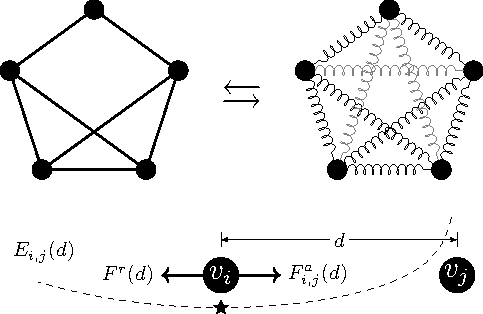
\includegraphics[height=5.5cm]{fr_layout/fr_layout.pdf}
  \caption{
    (Top) The illustration of the force model. Forces acts on every pairs of vertices.
    (Bottom) Forces $F_{i,j}^\mathrm{a}(d)$ and $F^\mathrm{r}(d)$ work between $v_i$ and $v_j$. The equilibrium of them is achieved at $d = k/\sqrt[3]{w_{i,j}}$, which equals $k$ when $w_{i,j} = 1$.
  }
  \label{fig:frLayout}
\end{figure}

We can also interrupt forces by its scalar potential~\cite{6183577}, in other words, energy $E_{i,j}: \bbR_{> 0} \to \bbR$, which is defined by
\begin{align}
  E_{i,j}^\mathrm{a}(d) & \defeq \int_{0}^{d} F_{i,j}^\mathrm{a}(r) \dd{r} = \frac{w_{i,j} d^3}{3k},\notag \\
  E^\mathrm{r}(d)       & \defeq \int_{\infty}^{d} F^\mathrm{r}(r) \dd{r} = -k^2\log{d}, \notag            \\
  E_{i,j}(d)            & \defeq E_{i,j}^\mathrm{a}(d) + E^\mathrm{r}(d). \label{eq:Eijr}
\end{align}
Although the energy function $E_{i,j}$ is convex and minimized when $d = k/\sqrt[3]{w_{i,j}}$, $E_{i,j}$ is not Lipschitz continuous since it diverges as $d \to 0$.
Plus, a function $x_i \mapsto E_{i,j}(\norm{x_i - x_j})$ is not convex for a fixed $x_j$. Refer to Fig.~\ref{fig:energy3d}.

\begin{figure}[t]
  \centering
  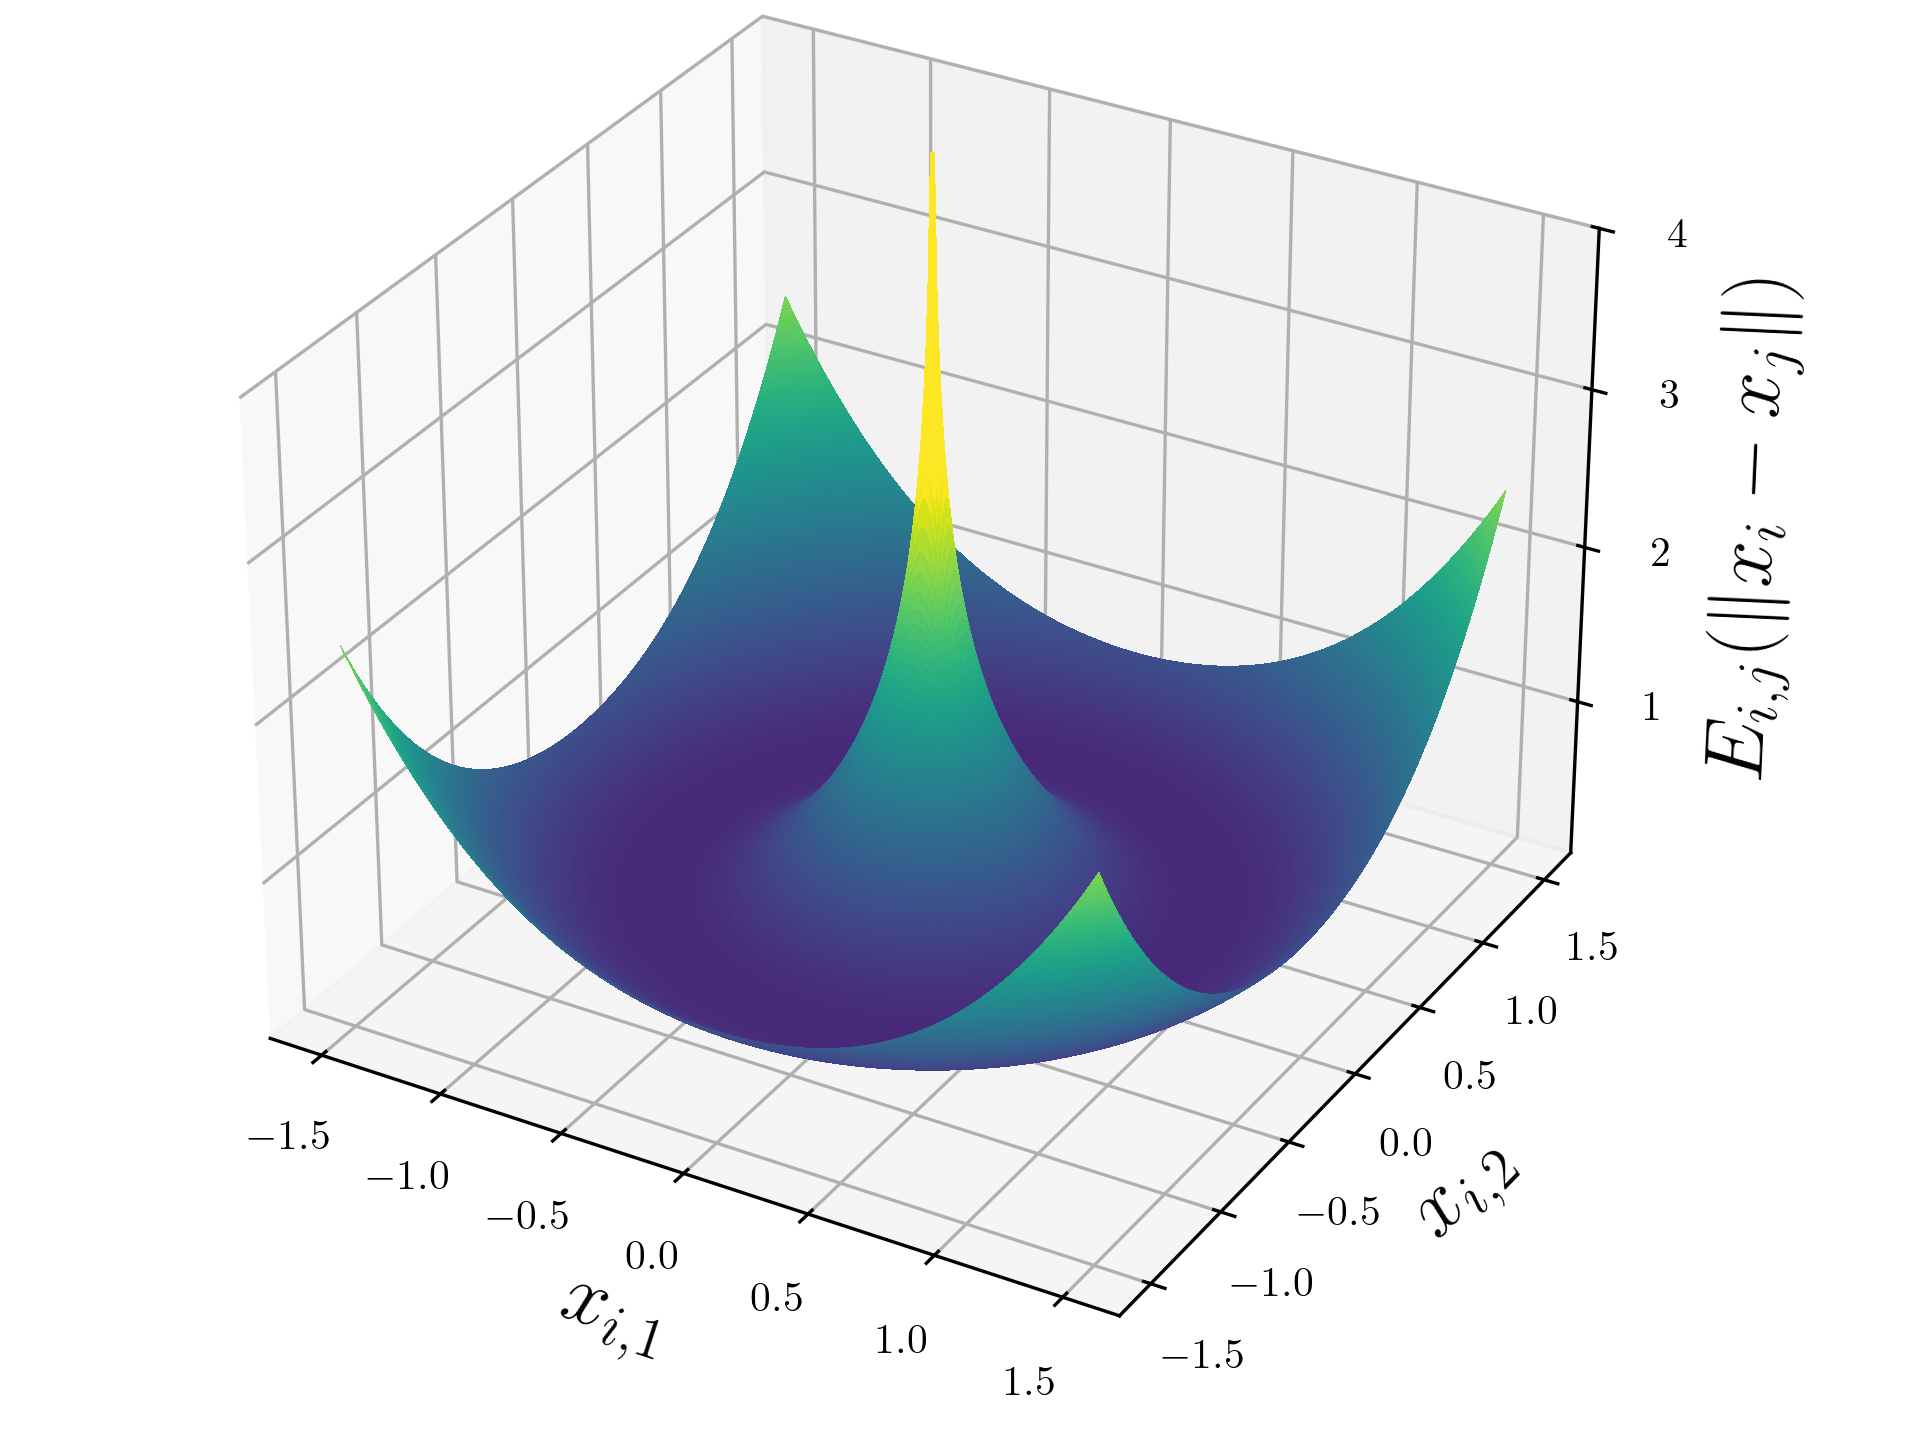
\includegraphics[height=4cm]{energy_3d/energy_3d.png}
  \caption{Energy function $E_{i,j}(\norm{x_i - x_j})$ for $x_i=(x_{i,1},x_{i,2})$, $x_j=(0,0), w_{i,j} = 1$ and $k = 1$. Although $E_{i,j}$ is convex as a function of $d = \norm{x_i - x_j}$, not convex as a function of $x_i$. As $x_i$ approaches $x_j$, the energy function diverges.}
  \label{fig:energy3d}
\end{figure}

Now, the optimization problem for the FR layout can be formulated as the minimization of the energy function $f: \bbR^{2 \times n} \to \bbR$, as known as the stress of the graph $G$:
\begin{mini}
  {X \in \bbR^{2 \times n}}
  {f(X) \defeq \sum_{i<j} E_{i,j}(\norm{x_i - x_j}).}
  {\label{eq:fr}}
  {}
\end{mini}
Seeking an equilibrium of the forces is equivalent to seeking a local minimum of the energy function $E_{i,j}$ for all pairs of vertices.
In the following, we will discuss how to optimize this minimization Prob.~\eqref{eq:fr}.

\subsection{Fruchterman--Reingold Algorithm}\label{ssec:frAlgorithm}

The Fruchterman--Reingold algorithm~\cite{fruchtermanGraphDrawingForcedirected1991} is the original force-directed algorithm and most standard approach for this force model.

Let denote $f_i: \bbR^2 \to \bbR$ as the energy function for the vertex $v_i$ at $x_i$. This is defined by
\begin{equation}\label{eq:fi}
  f_i(x_i) \defeq \sum_{j \neq i} E_{i,j}(\norm{x_i - x_j}),
\end{equation}
and its gradient, the sum of forces acting on the vertex $v_i$, is
\begin{equation}\label{eq:gradientFi}
  \nabla f_i(x_i) = \sum_{j \neq i} \qty(\frac{w_{i,j}\norm{x_i - x_j}}{k} - \frac{k^2}{\norm{x_i - x_j}^2}) (x_i-x_j),
\end{equation}

The pseudo-code of the FR algorithm is shown in Algorithm~\ref{alg:fr}, which can be regarded as a variant of gradient (steepest) descent method for the energy function $f$~\cite{tunkelang1999numerical}.
\begin{algorithm}[h]
  \caption{Fruchterman--Reingold algorithm}
  \label{alg:fr}
  \KwIn{Graph $G_W = (V, E)$}
  \KwOut{Point placement $X = (x_1, \dots, x_n)$}

  Define parameters $N_\mathrm{iter}^\mathsf{FR}, k, t, \Delta_t \defeq t/N_\mathrm{iter}^\mathsf{FR}$\;
  Define initial placement for all $v_i \in V$ randomly\;
  \For{$n_\mathrm{iter} \gets 1$ \KwTo $N_\mathrm{iter}^\mathsf{FR}$}{
    $\text{compute gradient } \nabla f_i(x_i)$ for all $v_i \in V$\;
    $x_i \gets x_i - t \frac{\nabla f_i(x_i)}{
        \norm{\nabla f_i(x_i)}}$ for all $v_i \in V$\;
    $t \gets t - \Delta_t$\;
    \If{\text{convergence condition is satisfied}}{
      \textbf{break}\;
    }
  }
  \Return $X$\;
\end{algorithm}
Alg.~\ref{alg:fr} is based on the original pseudo-code~\cite{fruchtermanGraphDrawingForcedirected1991} and implementation in NetworkX~\cite{hagberg2008exploring} with some omitted details.
The initial placement of the $n$ points are sampled from a uniform distribution on a unit square in general.
The parameter $t$ denotes the temperature, which governs the step size along the steepest descent. As the temperature gradually decreases, the algorithm converges to a particular placement, though this placement is not necessarily the optimal solution.

\subsection{L-BFGS Algorithm}\label{ssec:lbfgs}

\begin{figure}[t]
  \centering
  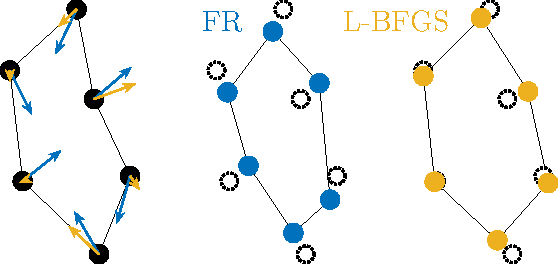
\includegraphics[height=3.59cm]{comparison/comparison_FRandLBFGS.pdf}
  \caption{
    Comparison of the FR algorithm and the L-BFGS algorithm.
    The FR algorithm moves vertices in a descent direction with a fixed step size (blue arrows), whereas the L-BFGS algorithm adjusts them differently since it utilizes approximated inverse Hessian (orange arrows).
  }
  \label{fig:comparisonFRandLBFGS}
\end{figure}

Another approach to solve the optimization Prob.~\eqref{eq:fr} is to use the Limited-memory Broyden--Fletcher--Goldfarb--Shanno (L-BFGS) algorithm~\cite{6183577}.
Using only a few recent gradient vectors, L-BFGS algorithm approximates the inverse Hessian of the objective function $f$, which is necessary to determine a descent direction~\cite{liuLimitedMemoryBFGS1989}.
We fix the maximum number of iterations to $N_\mathrm{iter}^{\mathsf{L-BFGS}}$.
L-BFGS is known to be very efficient for large-scale optimization problems, and the superior performance of the L-BFGS algorithm to the FR algorithm reported in Ref.\cite{6183577} also indicates this fact. Refer to Fig.~\ref{fig:comparisonFRandLBFGS} for a comparison to the FR algorithm.

For the optimization Prob.~\eqref{eq:fr}, we can apply the L-BFGS algorithm via flattening the matrix $X \in \bbR^{2 \times n}$ to a vector $\overline{X} \in \bbR^{2n}$.
However, it is worth noting that this method ignores the structure of $X$ and treats it just as a general optimization problem.
Thus, we can expect room for improvement by leveraging what we have ignored in this L-BFGS algorithm.

\subsection{Pre-Processing by Simulated Annealing}\label{ssec:preprocessing}

As a related work, we briefly introduce and discuss the pre-processing step proposed by Ref.~\cite{ghassemitoosiSimulatedAnnealingPreProcessing2016}.
Let $Q^\mathrm{circle} \defeq \qty{(\cos(2\pi i/n), \sin(2\pi i/n)) \mid 1 \leq i \leq n}$ be the points on a unit circle in $\bbR^2$.
For an unweighted graph $G_W$, let $E_2 \defeq \qty{\{v_i,v_j\} \mid \exists v_k \in V \st \{v_i,v_k\} \in E \land \{v_k,v_j\} \in E}~\setminus~E$ be a set of vertex pairs with a theoretical distance equal to 2.
This study defines the problem for pre-processing as
\begin{mini}
  {\pi\colon V \to Q^\mathrm{circle}}
  {\sum_{(i,j)\in E \cup E_2} \norm{\pi(v_i) - \pi(v_j)}^2,}
  {\label{eq:sa}}
  {}
  \addConstraint{\pi(v_i)}{\neq \pi(v_j),\quad}{\forall (i,j)~(i<j).}
\end{mini}
Prob.~\eqref{eq:sa} is a discrete optimization problem to find the best assignment $\pi$ from vertices $V$ to the points on the circle $Q^\mathrm{circle}$ just using Euclidean distances, not the energy functions.
By setting the result of Simulated Annealing (SA) for Prob.~\eqref{eq:sa} as the initial placement for the FR algorithm,  we can obtain a faster and better visualization.

However, the following limitations remain:
\begin{enumerate}
  \item Restricted to unweighted graphs.
  \item Confined to a simple circle layout, which could be ineffective for complex structure graphs.
  \item The only neighborhood in the SA is the random swapping of two vertices, making the optimization process inefficient for large-scale graphs.
  \item $\abs{E_2}$ could be $\Theta(n^2)$, unable to leverage the sparsity of graphs if it exists.
\end{enumerate}
Although our algorithm and motivation is different from this study's, we are dealing with these limitations and can regard our study as an extension of this prior work.

\section{Proposed Algorithm}\label{sec:algorithm}

In this section, we propose a new initial placement algorithm for the FR layout.
We first introduce the graph drawing by Stochastic Gradient Descent (SGD)~\cite{8419285} and the concept of the coordinate Newton direction, the key concepts of our research.
Then, we define the discrete optimization problem for initial placement and propose a new algorithm to optimize it.

\subsection{Related Work}\label{ssec:relatedWork}

Firstly, we introduce two important previous works. Although these works are not completely same as our work, explaining them is quite helpful to understand the motivation of our work.

\subsubsection{Graph Drawing by Stochastic Gradient Descent}\label{ssec:sgd}

When we regard graph drawing as an optimization problem, Stochastic Gradient Descent (SGD) for Kamada--Kawai (KK) layout~\cite{kamadaAlgorithmDrawingGeneral1989} is one of the most notable works.
In KK layout, we regard $G$ as a complete graph and assign the energy function $E_{i,j}$ to all edges.
SGD in this context means to repeat randomly selecting a edge $\{v_i,v_j\}$ and updating $x_i$ and $x_j$ with the gradient of $E_{i,j}$. This algorithm is known to be effective various optimization problems in general, and its effectiveness for graph drawing is shown in Ref.~\cite{8419285}.

Although applying SGD to our problem Prob.~\eqref{eq:fr} is straightforward, it is not effective for this problem.
This is because the force model we consider assigns exactly the same function $E_{i,j}(d)=-k^2\log{d}$ to all $(i,j)$ such that $w_{i,j}=0$. Optimizing $E_{i,j}$ only increases the distance between vertices $v_i$ and $v_j$, no matter how close they are in the optimal solution. Thus, the gradient of $E_{i,j}$ is not informative enough to find the optimal solution, and we need to develop a new optimization method for Prob.~\eqref{eq:fr}.

Still, the idea to randomly select a edge and update its position is quite suggestive. Based on this idea, we propose to randomly select a vertex and update its position.

\subsubsection{Newton Direction and Subspace Newton Direction}\label{ssec:introNewton}

We also introduce the Newton direction.
Let $f: \bbR^n \to \bbR$ be a convex function.
The second order approximation at $x_0$ is
\begin{equation*}
  f(x_0) + \nabla f(x_0)^\top (x - x_0) + \frac{1}{2} (x - x_0)^\top \nabla^2 f(x_0) (x - x_0).
\end{equation*}
Since $f$ is convex, the Hessian matrix $\nabla^2 f(x_0)$ is positive semi-definite.
The argmin $x^*$ of this approximation satisfies
\begin{align*}
       & \nabla f(x_0) + \nabla^2 f(x_0) (x^* - x_0) = 0 \\
  \iff & x^* = x_0 - \nabla^2 f(x_0)^{-1} \nabla f(x_0).
\end{align*}
We call the direction $d = -\nabla^2 f(x_0)^{-1} \nabla f(x_0)$ as the Newton direction.
Although Newton direction is the optimal direction for the approximated $f$, it requires the computation of the inverse Hessian $\nabla^2 f(x_0)^{-1} \in \bbR^{n \times n}$, posing a high computational cost for large-scale problems. Actually, the reason why L-BFGS algorithm approximates the inverse Hessian is to avoid this computational cost.

Still, we can leverage the concept of the Newton direction in a different way, the coordinate Newton direction.
Instead of computing the inverse Hessian $\nabla^2 f(x_0)^{-1}$ in the entire variable space $\bbR^n$, we limit the variable $x$ to its coordinate block $x_i$ with fewer dimensions, and compute $\nabla^2 f_i(x_i)^{-1} \nabla f_i(x_i)$ where $f_i$ is a restricted function of $f$ to $x_i$.
Since the computation of the coordinate Newton direction is much cheaper than that of the Newton direction, we can repeat this procedure many times.
In general, this idea is also known as Randomized Subspace Newton (RSN)~\cite{NEURIPS2019_bc6dc48b} in a broader context.

In particular, this coordinate Newton direction has obvious natural affinity to the Prob.~\eqref{eq:fr} in Sec.~\ref{ssec:preprocessing}.
By taking $x_i$, the position of the vertex $v_i$, as the coordinate block, we can compute the Newton direction of $f_i$ in~Eq.~\eqref{eq:fi}.
Although directly applying this idea to Prob.~\eqref{eq:fr} is challenging as we will discuss in Sec.~\ref{sec:challenges}, we leverage this coordinate Newton direction to propose our algorithm.

\subsection{Reduction To The Discrete Optimization Problem}\label{ssec:reduction}

Now, to define a problem for our initial placement, we transform the optimization problem \eqref{eq:fr} into a constrained discrete optimization problem.
As written in Sec.~\ref{ssec:sgd}, the energy function $E_{i,j}$ is $-k^2\log{d}$ for all $(i,j) \notin E$.
Considering the sparsity of many practical graphs $(\abs{E} \ll \abs{V}^2)$, simplifying as follow is reasonable:
\begin{mini}
  {X \in \bbR^{2 \times n}}
  {\sum_{(i,j)\in E} \frac{w_{i,j}\norm{x_i - x_j}^3}{3k}- \sum_{i<j} k^2\log{\norm{x_i - x_j}}.}
  {\label{eq:frApprox}}
  {}
\end{mini}
Further, by converting the second term into a constraint, the problem \eqref{eq:frApprox} can be approximated so that the objective function can be computed with a complexity dependent on $\abs{E}$ rather than $\abs{V}^2$:
\begin{mini}
  {X \in \bbR^{2 \times n}}
  {f^{\mathrm{a}}(X) \defeq \sum_{(i,j)\in E} \frac{w_{i,j}\norm{x_i - x_j}^3}{3k}}
  {\label{eq:frApprox2}}
  {}
  \addConstraint{\norm{x_i - x_j}}{\geq \epsilon,\quad}{\forall (i,j)\,(i<j)}
\end{mini}
where $\epsilon$ is a suitably chosen positive constant. This conversion does not lose the essence of the problem too much because $E^\mathrm{r}(d)=-k^2\log{d}$ is a convex function such that it decreases monotonically concerning $d$. Thus, for sufficiently large $d$, the value of $-k^2\log{d}$ does not grow excessively, and for too small $d$, we can prevent the divergence of the energy function by setting $\epsilon$.

However, problem \eqref{eq:frApprox2} still involves $\order{\abs{V}^2}$ constraints, which negates the advantage of computing the objective function with $\order{\abs{E}}$ complexity.
To further simplify, we incorporate the concept of initial placements as mentioned in Sec.~\ref{ssec:preprocessing}.
By simplifying problem \eqref{eq:frApprox2} with a fixed initial placement $Q$ whose points are separated by at least $\epsilon$, we obtain the following discrete optimization problem:
\begin{mini}
  {\pi: V \to Q}
  {\sum_{(i,j)\in E} \frac{w_{i,j}\norm{\pi(v_i) - \pi(v_j)}^3}{3k},}
  {\label{eq:frApprox3}}
  {}
  \addConstraint{\pi(v_i)}{\neq \pi(v_j),\quad}{\forall (i,j)~(i<j).}
\end{mini}
It means that with a discrete set of points $Q$ such that the points are separated by at least $\epsilon$, we seek the best injection $\pi :V \to Q$ that minimizes the objective function $f^{\mathrm{a}}$.
By fixing the possible point placement in advance, we can skip the check of the $\order{\abs{V}^2}$ constraints, reducing the computational complexity to $\order{\abs{E}}$ and thus offering significant speedup.
See Fig.~\ref{fig:pi} as a visual explanation.

\begin{figure}[t]
  \centering
  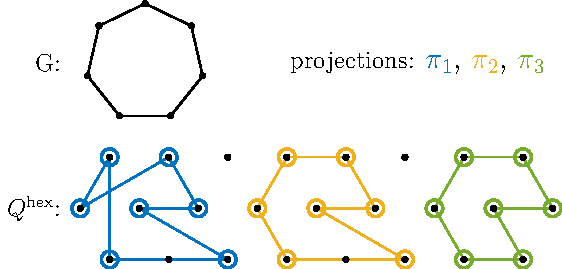
\includegraphics[width=\columnwidth]{pi/pi.pdf}
  \caption{
    Concept of $Q$ and $\pi$.
    The injection $\pi$ maps vertices $V$ to a discrete point placement $Q$, especially a hexagonal lattice $Q^\mathrm{hex}$.
    Apparently, among $\pi_1, \pi_2, \pi_3$, the right one $\pi_3$ is the best mapping for the Prob.~\eqref{eq:frApprox3}.
  }
  \label{fig:pi}
\end{figure}

As an instance of such a discrete point placement $Q$, we can consider various types of placements, including $Q^\mathrm{circle}$~\cite{ghassemitoosiSimulatedAnnealingPreProcessing2016}.
However, in this study, we adopt a hexagonal lattice $Q^\mathrm{hex}$~\cite{patelHexagonalGrids2013,s22145179}.
When minimizing the attraction energy $f^\mathrm{a}$, it is advantageous for the points to cluster as closely as possible. In this context, the hexagonal lattice is known for its densest packing structure in space with the least distance $\epsilon$ between points and offers computational simplicity. Thus, $Q^\mathrm{hex}$ is a suitable choice for our purpose.

\subsection{Newton Direction for Discrete Optimization}\label{ssec:newtonDirection}

Next, using the coordinate Newton direction of a randomly selected vertex, as mentioned in Sec.~\ref{ssec:relatedWork}, we optimize the discrete optimization problem.

Let the objective function $f^{\mathrm{a}}_i(x_i)$ corresponding to a vertex $v_i$ be
\begin{equation*}
  f^{\mathrm{a}}_i(x_i) \defeq \sum_{j \neq i} \frac{w_{i,j}\norm{x_i - x_j}^3}{3k}.
\end{equation*}
Its gradient and Hessian matrix are
\begin{align*}
  \nabla f^{\mathrm{a}}_i(x_i)   & = \sum_{j \neq i} \frac{w_{i,j}\norm{x_i - x_j}}{k} (x_i - x_j),                     \\
  \nabla^2 f^{\mathrm{a}}_i(x_i) & = \sum_{j \neq i} \frac{w_{i,j}\norm{x_i - x_j}}{k} \mqty(1                      & 0 \\0&1) \\
                                 & + \sum_{j \neq i} \frac{w_{i,j}}{k\norm{x_i - x_j}} (x_i - x_j)(x_i - x_j)^\top.
\end{align*}
Since $f^{\mathrm{a}}_i$ is convex, the Hessian matrix $\nabla^2 f^{\mathrm{a}}_i(x_i)$ is positive semi-definite. This is a large difference from the functions $f_i(x_i)$ in Eq.~\eqref{eq:fi} and $f^{\mathrm{a}}(X)$ in Prob.~\eqref{eq:frApprox2}, which are not convex.

The ordinary updated rule with the coordinate Newton direction is
\begin{equation*}
  x_i - \nabla^2 f^{\mathrm{a}}_i(x_i)^{-1} \nabla f^{\mathrm{a}}_i(x_i).
\end{equation*}
However, $x_i^\mathrm{new}$ may not be in the hexagonal lattice $Q^\mathrm{hex}$, which is a constraint of Prob.~\eqref{eq:frApprox3}.
Thus, we need to round to the nearest point in $Q^\mathrm{hex}$. Plus, we empirically found that adding a random vector to the Newton direction is effective for the optimization process, which is a similar strategy to the SA in Sec.~\ref{ssec:preprocessing}. This randomness can help to escape from local minima and to explore the solution space more effectively.
In conclusion, the updated rule for the vertex $v_i$ is
\begin{equation*}
  x_i^\mathrm{new} \gets \mathrm{round}\qty(x_i - \nabla^2 f^{\mathrm{a}}_i(x_i)^{-1} \nabla f^{\mathrm{a}}_i(x_i) + t \cdot \text{rand}),
\end{equation*}
where $\mathrm{round}(\hat{x})$ denotes the operation assigning $\hat{x}$ to the nearest point in the hexagonal lattice $Q^\mathrm{hex}$, $\mathrm{rand}$ is a random vector with a unit norm, and $t$ is a parameter controlling the randomness.

If there is a vertex $v_j$ such that $\pi(v_j) = x_i^\mathrm{new}$, we swap the vertices $v_i$ and $v_j$ in $\pi$ to keep the injective property of $\pi$. Otherwise, we just update $\pi(v_i)$ to $x_i^\mathrm{new}$. Refer to Fig.~\ref{fig:hex} for a visual explanation.

\begin{figure}[t]
  \centering
  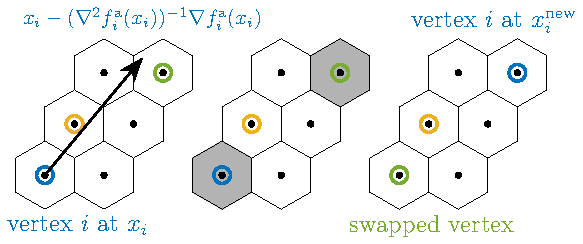
\includegraphics[width=\columnwidth]{hex/hex.pdf}
  \caption{Visual explanation of the one iteration of the proposed algorithm. Step1. Compute the coordinate Newton direction for a randomly selected vertex (blue). Step2. Decide $x_i^\mathrm{new}$ by rounding the direction and adding a random vector. Step3. Swap the vertices if there is a collision. In this case, swap blue and green vertices.}
  \label{fig:hex}
\end{figure}

\subsection{Optimal Scaling}\label{ssec:optimalScaling}

When we optimize a placement for FR-layout with an initial placement obtained, scaling the initial placement at first can often yield better results than directly using the unmodified initial placement.
In this subsection, we explain how to find the optimal scaling factor that minimizes the energy function for a given placement.

Let us formulate the optimization problem for the scaling factor $c \in \bbR_{> 0}$.
For an initial placement $X = (x_1, \dots, x_n)$, we rescale it as $x_i \gets c x_i$ for all $i$.
This problem is to minimize the energy function $\phi(c)$ defined by
\begin{align*}
  \phi(c) \defeq {} & \qty(\sum_{(i,j) \in E} \frac{w_{i,j} (c \norm{x_i - x_j})^3}{3k}) - k^2 \sum_{i < j} \log(c \norm{x_i - x_j})     \\
  \begin{split}
    = {} & c^3 \qty(\sum_{(i,j) \in E} \frac{w_{i,j} \norm{x_i - x_j}^3}{3k}) - k^2 n(n-1)\log(c) \\
         & - k^2 \sum_{i < j} \log(\norm{x_i - x_j}),
  \end{split} \\
  \phi'(c) = {}     & 3c^2 \qty(\sum_{(i,j) \in E} \frac{w_{i,j} \norm{x_i - x_j}^3}{3k}) - \frac{k^2 n(n-1)}{c}.
\end{align*}
The function $\phi(c)$ is convex, and we can find the optimal scaling factor $c^*$ by solving $\phi'(c^*) = 0$, which yields
\begin{equation}\label{eq:scaling}
  c^* = \qty(\frac{k^2 n(n-1)}{3 \sum_{(i,j) \in E} \frac{w_{i,j} \norm{x_i - x_j}^3}{k}})^{1/3}.
\end{equation}
This value can be computed in $\order{\abs{E}}$ complexity.
Using this scaling factor, we can obtain a further better initial placement for the FR layout.

It is notable that the optimal solution to Prob.~\eqref{eq:frApprox3} is invariant under scaling, thus we can select any $\epsilon$ to define the hexagonal lattice $Q^\mathrm{hex}$ as far as we scale the placement by $c^*$ as post-processing.

\subsection{Pseudo Code}\label{ssec:pseudoCode}

We presented the overall framework of the proposed method in Algorithm~\ref{alg:proposed}.
Be aware that the proposed algorithm is not a complete solution to Prob.~\eqref{eq:fr}, this only provides an initial placement for the algorithms such as the FR algorithm or the L-BFGS algorithm.

\begin{algorithm}[h]
  \caption{Proposed algorithm as initial placement for the FR layout}
  \label{alg:proposed}
  \KwIn{Graph $G_W = (V, E)$, subspace dimension $s$}
  \KwOut{Point placement $X = (x_1, \dots, x_n)$}

  Define parameters $N_\mathrm{iter}^\mathsf{CN}, k, t, \Delta t$ and hexagonal lattice $Q^\mathrm{hex}$\;
  Set $\pi$ as a injection from $V$ to $Q^\mathrm{hex}$ randomly\;
  \For{$j \gets 0$ \KwTo $N_\mathrm{iter}^\mathsf{CN}$}{
  $v_i \gets \text{randomly selected vertex from } V$\;
  $x_i \gets \pi(v_i)$\;
  $x_i^\mathrm{new} \gets \mathrm{round}(x_i - \nabla^2 f_i(x_i)^{-1} \nabla f_i(x_i) + t \cdot \mathrm{rand})$\;
    \If{$\exists v_j \st \pi(v_j) = x_i^\mathrm{new}$}{
      Swap $v_i$ and $v_j$ in $\pi$\;
    } \Else{
      $\pi(v_i) \gets x_i^\mathrm{new}$\;
    }
    }
  $x_i \gets \pi(v_i)$ for all $v_i \in V$\;
  $c^* \gets \text{optimal scaling factor by Eq.~\eqref{eq:scaling}}$\;
  $x_i \gets c^* x_i$ for all $v_i \in V$\;
    \Return $X$
\end{algorithm}

\subsection{Alternative Approach}\label{ssec:alternative}

As the end of this section, we explain an alternative approach of this algorithm. We can also consider to update all vertices simultaneously, not one by one.
It means that moving all the points $\{x_i\}_{1 \leq i \leq \abs{V}} \subseteq Q^\mathrm{hex}$ on the hexagonal grid to arbitrary points $\{\hat{x}_i \defeq x_i - \nabla^2 f_i(x_i)^{-1} \nabla f_i(x_i) \}_{1 \leq i \leq \abs{V}} \subseteq \bbR^2$, and then assign all these $\abs{V}$ points to the nearest points in $Q^\mathrm{hex}$.
If we define the assignment problem as the minimization of the sum of the squared distances between $\{x_i\}_{1 \leq i \leq \abs{V}}$ and $\{\hat{x}_i\}_{1 \leq i \leq \abs{V}}$, we can solve this problem by minimum-cost flow or Hungarian algorithm with $\order{\abs{V}^3}$ complexity.
Additionally, we can obtain a heuristic solution in $\order{\abs{V} \log \abs{V}}$ by appropriately sorting $\{\hat{x}_i^\mathrm{new}\}_{1 \leq i \leq \abs{V}}$.

While we are not expecting as good performances as the proposed algorithm, they offer certain advantages, such as simplified implementation or avoiding random access to arrays.

\section{Numerical Experiment} \label{sec:experiment}

\begin{figure*}[t]
  \centering
  \begin{minipage}{\columnwidth}
    \centering
    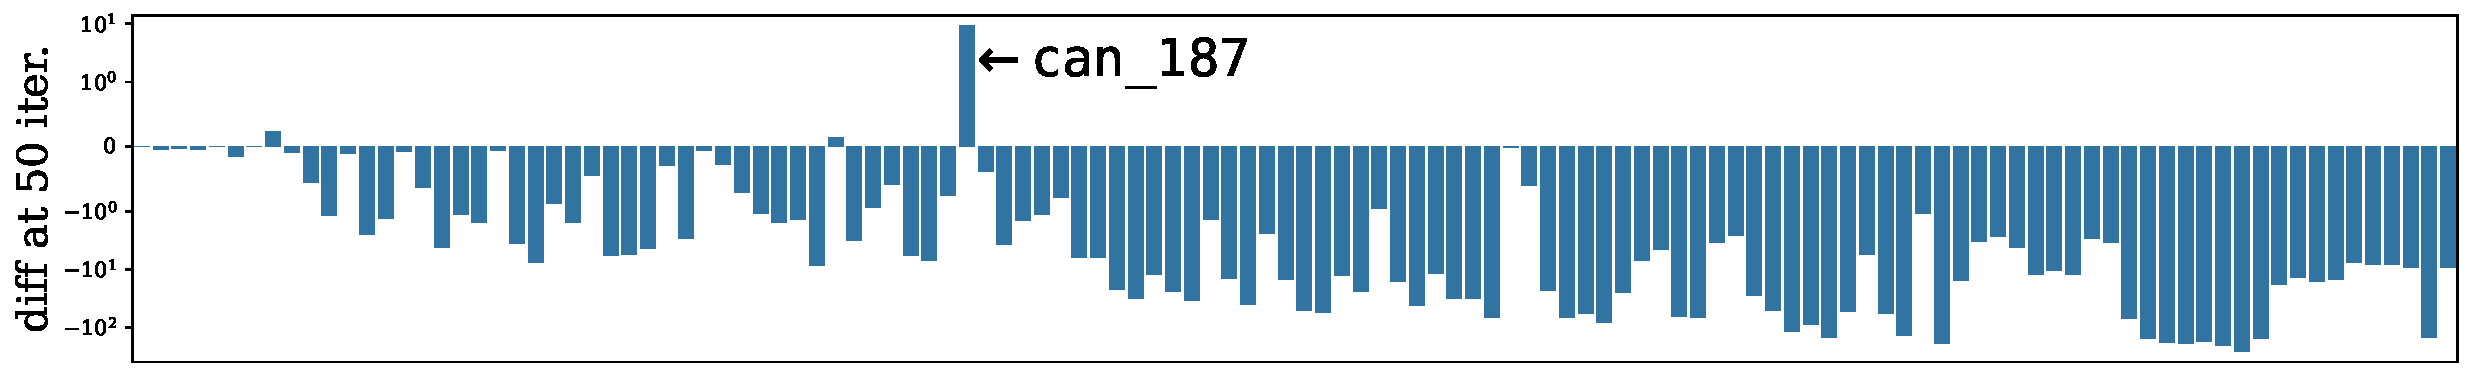
\includegraphics[width=\columnwidth]{overall/plot/diff_FR_50.pdf}
  \end{minipage}
  \begin{minipage}{\columnwidth}
    \centering
    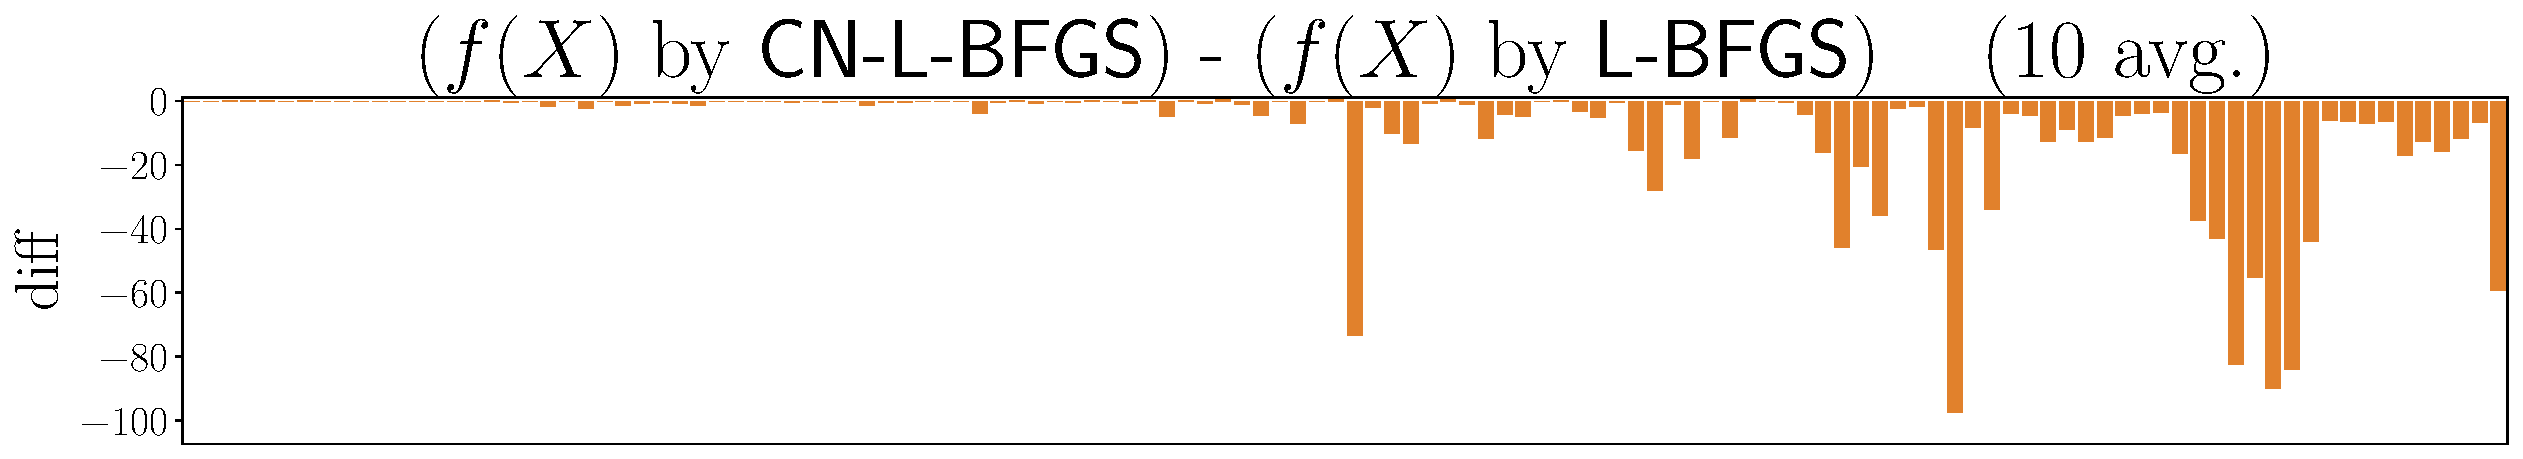
\includegraphics[width=\columnwidth]{overall/plot/diff_L-BFGS_50.pdf}
  \end{minipage}
  \caption{
    Comparison of the proposed initialization with random initialization.
    For non-\textsf{CN} algorithms, $N_\mathrm{iter}^\mathsf{FR}$ and $N_\mathrm{iter}^\mathsf{L-BFGS}$ as 50, the default parameter of NetworkX~\cite{hagberg2008exploring}.
    For \textsf{CN} algorithms, we set them as 45, since it contains pre-processing step.
    Almost all of the cases, the difference are negative, meaning that the proposed algorithm performed faster and better than random initialization.
  }
  \label{fig:diff_L_BFGS}
\end{figure*}

\begin{figure}[t]
  \centering
  \begin{minipage}{0.49\columnwidth}
    \centering
    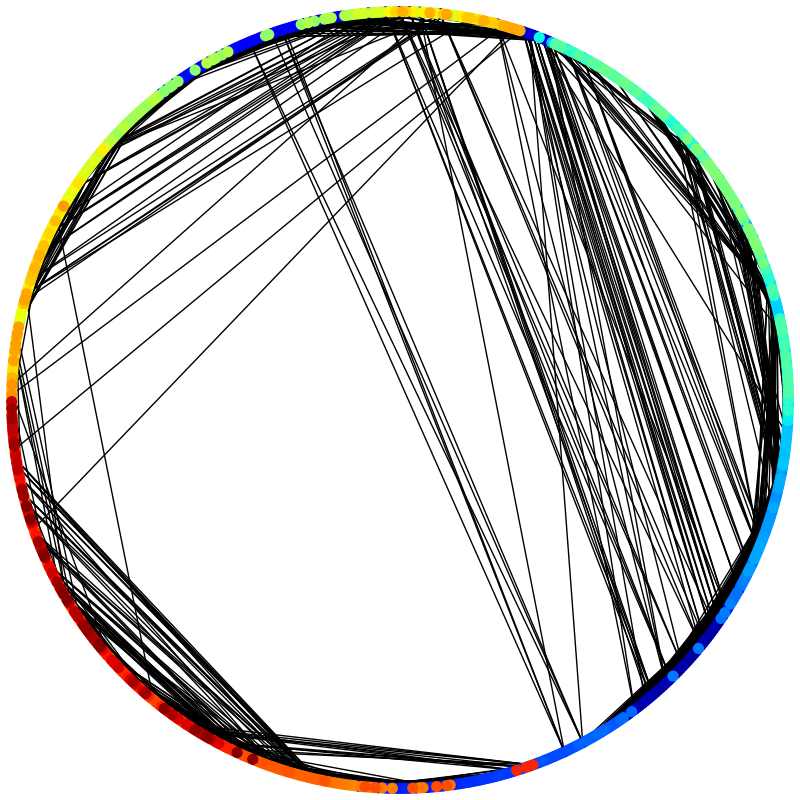
\includegraphics[width=\columnwidth]{circle/vis/can_715_CI-L-BFGS_50_first.png}
  \end{minipage}
  \begin{minipage}{0.49\columnwidth}
    \centering
    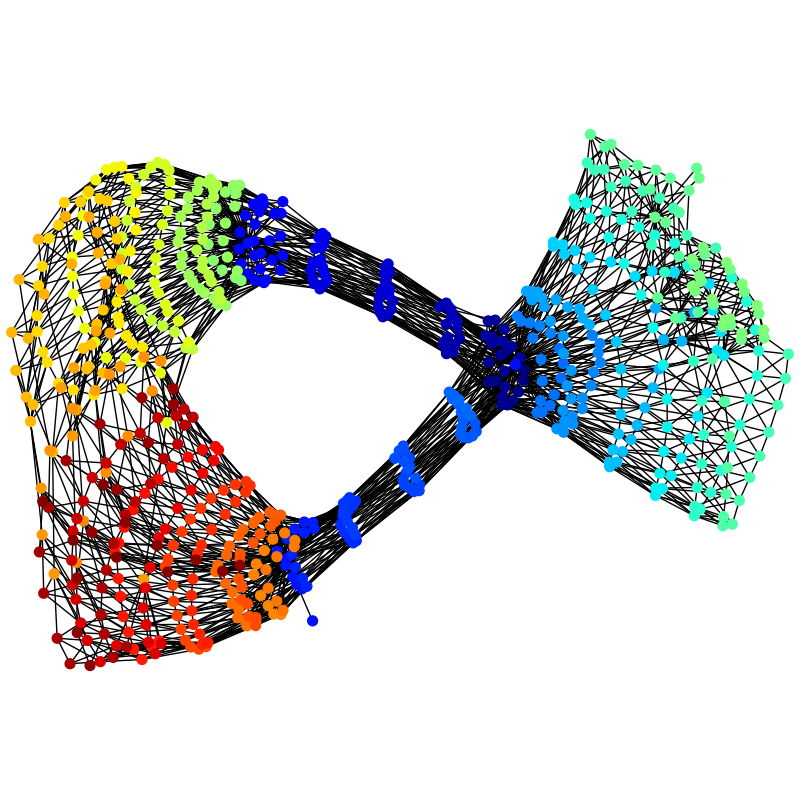
\includegraphics[width=\columnwidth]{circle/vis/can_715_CI-L-BFGS_50_last.png}
  \end{minipage}
  \caption{\texttt{can\_715} with \textsf{CI-L-BFGS}}
  \label{fig:can_715_CI}
\end{figure}
\begin{figure}[t]
  \centering
  \begin{minipage}{0.49\columnwidth}
    \centering
    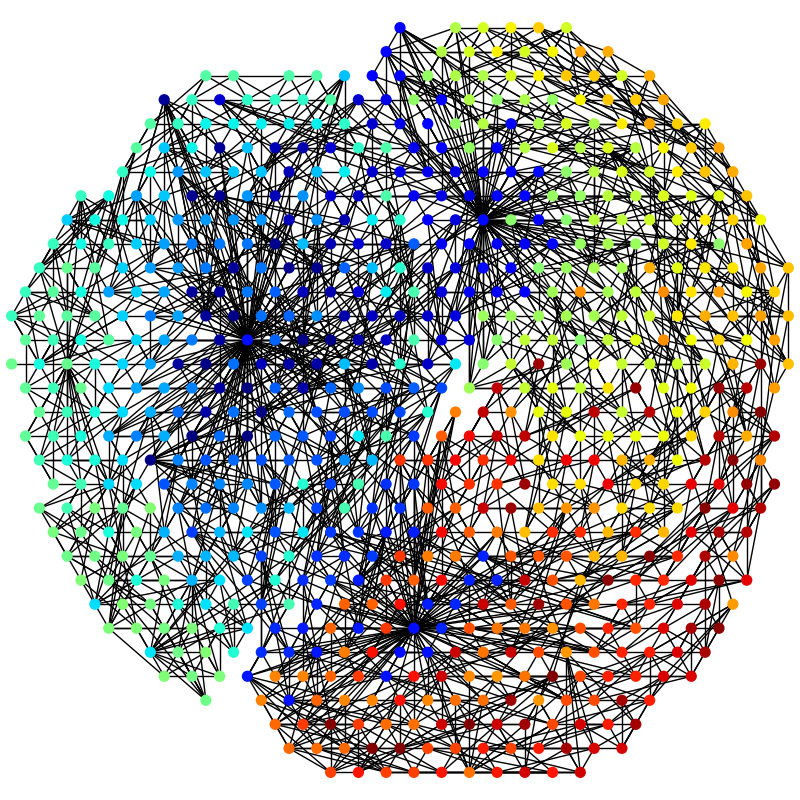
\includegraphics[width=\columnwidth]{circle/vis/can_715_CN-L-BFGS_50_first.png}
  \end{minipage}
  \begin{minipage}{0.49\columnwidth}
    \centering
    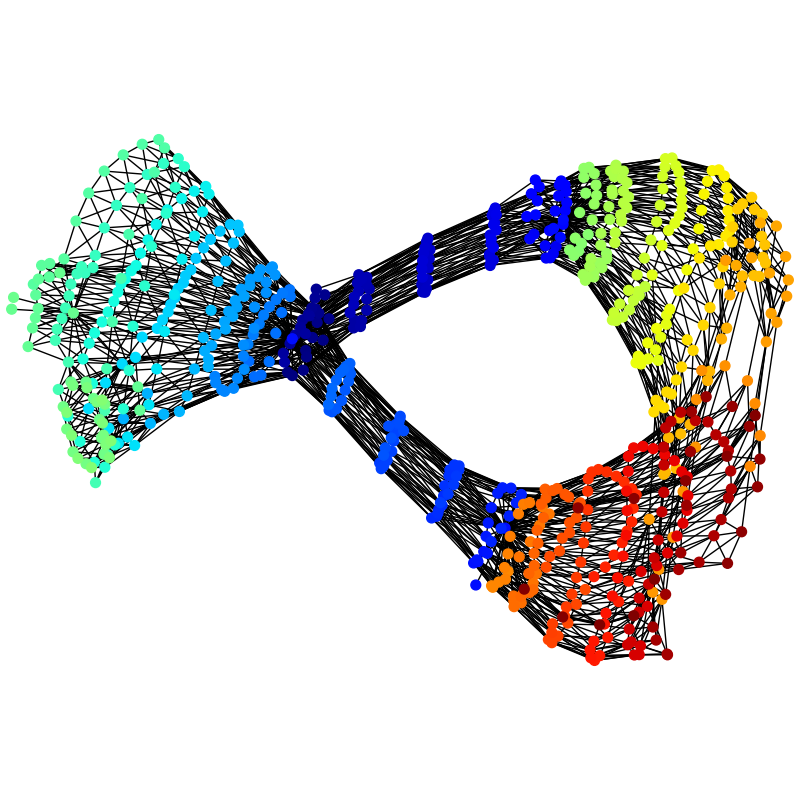
\includegraphics[width=\columnwidth]{circle/vis/can_715_CN-L-BFGS_50_last.png}
  \end{minipage}
  \caption{\texttt{can\_715} with \textsf{CN-L-BFGS}}
  \label{fig:can_715_CN}
\end{figure}
\begin{figure}[t]
  \centering
  \begin{minipage}{0.49\columnwidth}
    \centering
    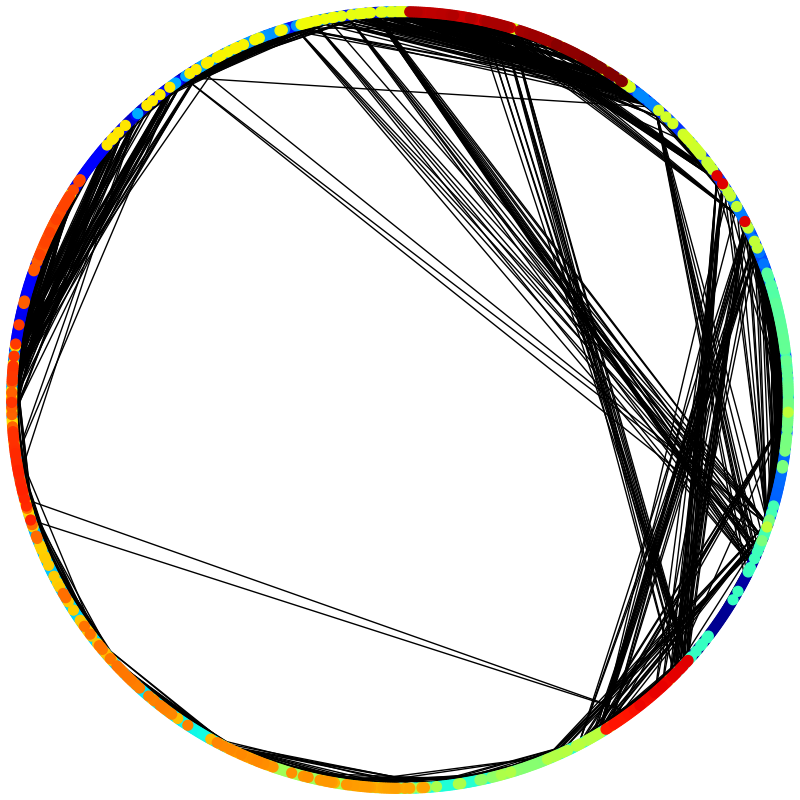
\includegraphics[width=\columnwidth]{circle/vis/collins_15NN_CI-L-BFGS_50_first.png}
  \end{minipage}
  \begin{minipage}{0.49\columnwidth}
    \centering
    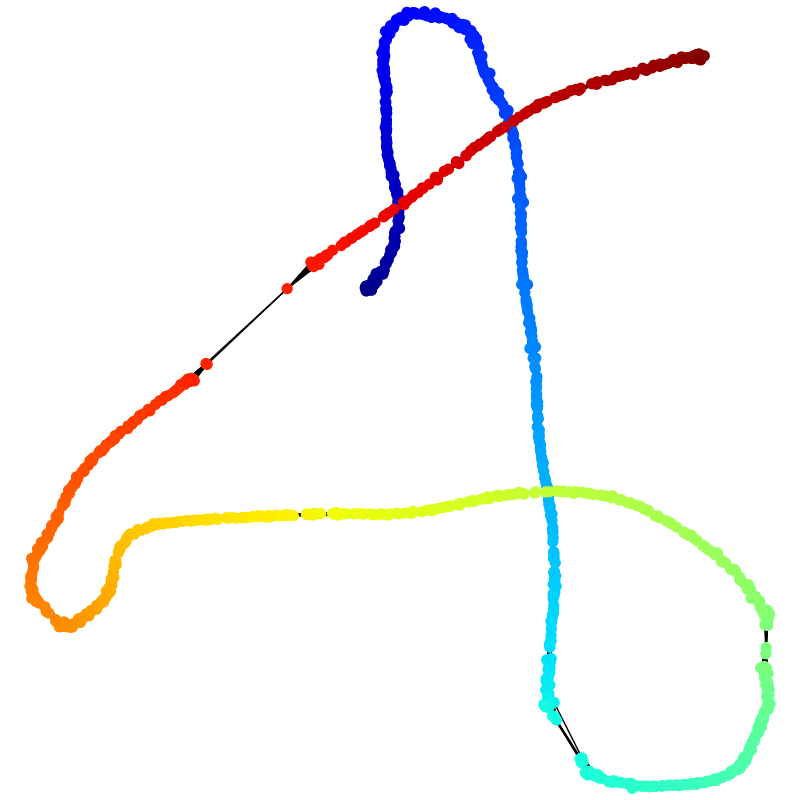
\includegraphics[width=\columnwidth]{circle/vis/collins_15NN_CI-L-BFGS_50_last.png}
  \end{minipage}
  \caption{\texttt{collins\_15NN} with \textsf{CI-L-BFGS}}
  \label{fig:collins_15NN_CI}
\end{figure}
\begin{figure}[t]
  \centering
  \begin{minipage}{0.49\columnwidth}
    \centering
    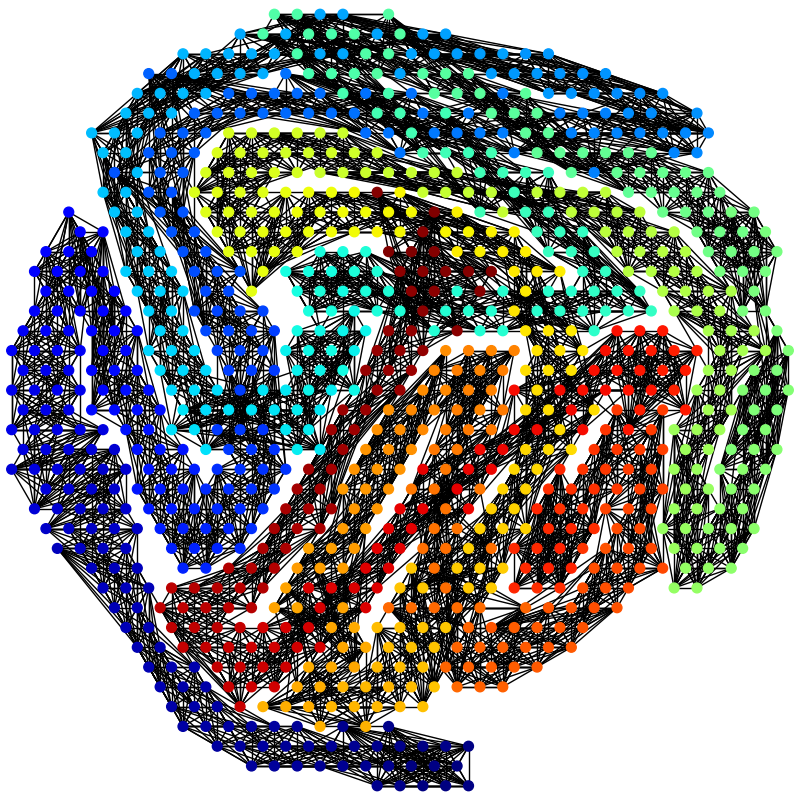
\includegraphics[width=\columnwidth]{circle/vis/collins_15NN_CN-L-BFGS_50_first.png}
  \end{minipage}
  \begin{minipage}{0.49\columnwidth}
    \centering
    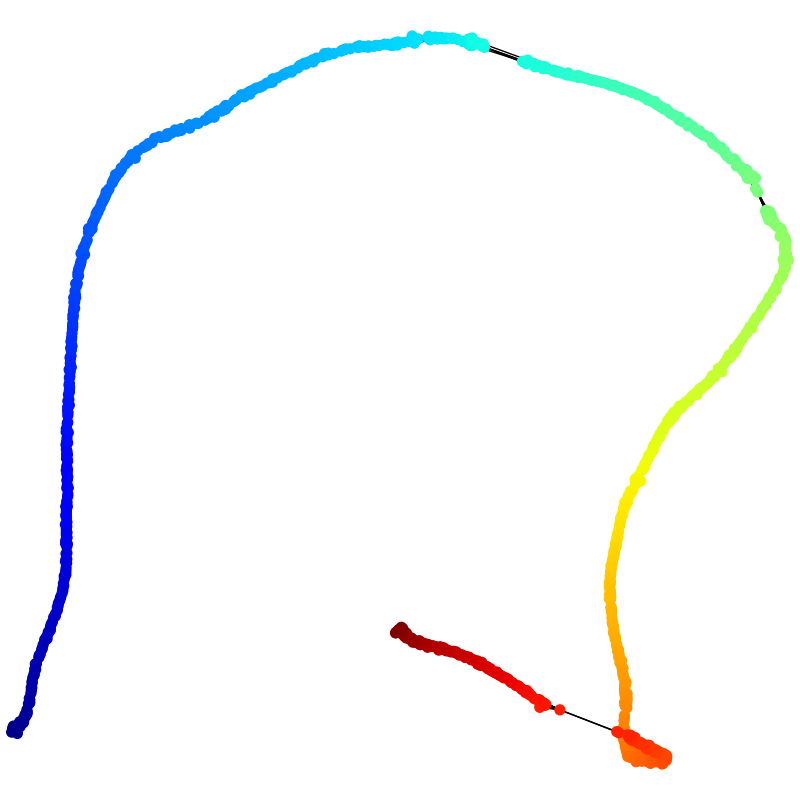
\includegraphics[width=\columnwidth]{circle/vis/collins_15NN_CN-L-BFGS_50_last.png}
  \end{minipage}
  \caption{\texttt{collins\_15NN} with \textsf{CN-L-BFGS}}
  \label{fig:collins_15NN_CN}
\end{figure}

In this section, we evaluate the proposed algorithm by various numerical experiments based on the setup described in Sec.~\ref{ssec:setup}.
We conducted two types of experiments, based on Ref.~\cite{8419285}:
exhaustive experiments to evaluate the performance of the proposed algorithm in various situations in Sec.~\ref{ssec:exprAll},
and detailed experiments to investigate the behavior of the proposed algorithm in detail in Sec.~\ref{ssec:exprDetail}.

\subsection{Experimental Setup}\label{ssec:setup}

All numerical experiments in this section were conducted using \Cpp17 compiled by GCC 10.5.0 on a laptop computer powered by Intel(R) Core(TM) i7-10510U CPU with 16 GB RAM.

To implement FR algorithm and L-BFGS algorithm, we referenced NetworkX version 3.3~\cite{hagberg2008exploring}, SciPy 1.14.1 ~\cite{2020SciPy-NMeth}, and C++ L-BFGS~\cite{qiuYixuanLBFGSpp2024,okazakiChokkanLiblbfgs2024}. In particular, we used almost the same parameters as NetworkX's \textsf{spring\_layout} for the FR algorithm.
We also referenced the open-source code of the hexagonal grid from~\cite{patelHexagonalGrids2013}.
As a side note, we also used Graphviz version 2.43.0~\cite{ellsonGraphvizOpenSource2002} to draw Fig.~\ref{fig:cycle}.

We used the 4 algorithms: FR algorithm (\textsf{FR}), the proposed initialization plus FR algorithm (\textsf{CN-FR}), L-BFGS algorithm (\textsf{L-BFGS}), and the proposed initialization plus L-BFGS algorithm (\textsf{CN-L-BFGS}). \textsf{CN} represents the Subspace Newton, and we refer \textsf{CN-FR} and \textsf{CN-L-BFGS} as \textsf{CN}, and \textsf{FR} and \textsf{L-BFGS} as non-\textsf{CN}.

As a parameter, we used $N_\mathrm{iter}^\mathsf{CN} = 3 \frac{\abs{V}^3}{\abs{E}}$ for the FR algorithm. Since the amortized time complexity per iteration of
Algorithm~\ref{alg:proposed} is $\order{\frac{\abs{E}}{\abs{V}}}$, we can roughly expect that the computational time of the proposed algorithm is equivalent to 3 iterations of the FR algorithm.

All the codes are available at our GitHub~\cite{ThisPaperGitHub}.

\subsection{Exhaustive Experiment}\label{ssec:exprAll}

To begin with, we conducted an exhaustive experiment to evaluate the performance of the proposed algorithm with various graphs.

As a dataset, we used matrices from Sparse Matrix Collection~\cite{davis2011university} satisfying the condition~\eqref{eq:WCondition} with $\abs{V} \leq 1000$, in total 124 graphs.

The result is shown in Fig.~\ref{fig:individual}.
Almost all of the cases, the proposed algorithm performed better than random initialization.

There are a few cases where the proposed algorithm performed worse than random initialization, and we visualized such cases in Fig.~\ref{fig:can_187}, Fig.~\ref{fig:can_73}, Fig.~\ref{fig:iris_dataset_30NN}, and Fig.~\ref{fig:dwt_592}.
We can observe that the reasons why it was worse though these figures. \orange{todo}

\subsection{detailed Experiment}\label{ssec:exprDetail}

\begin{figure*}[btp]
  \centering
  \addtolength{\tabcolsep}{-0.5em}
  \begin{tabular}{cccccc}
    \multicolumn{6}{c}{\textbf{\texttt{cycle300}} $(\abs{V}=300, \abs{E}=300, \text{sparsity}=0.669\text{\%}) \quad Figures are at 150 iterations.$}     \\
    \raisebox{-.5\height}{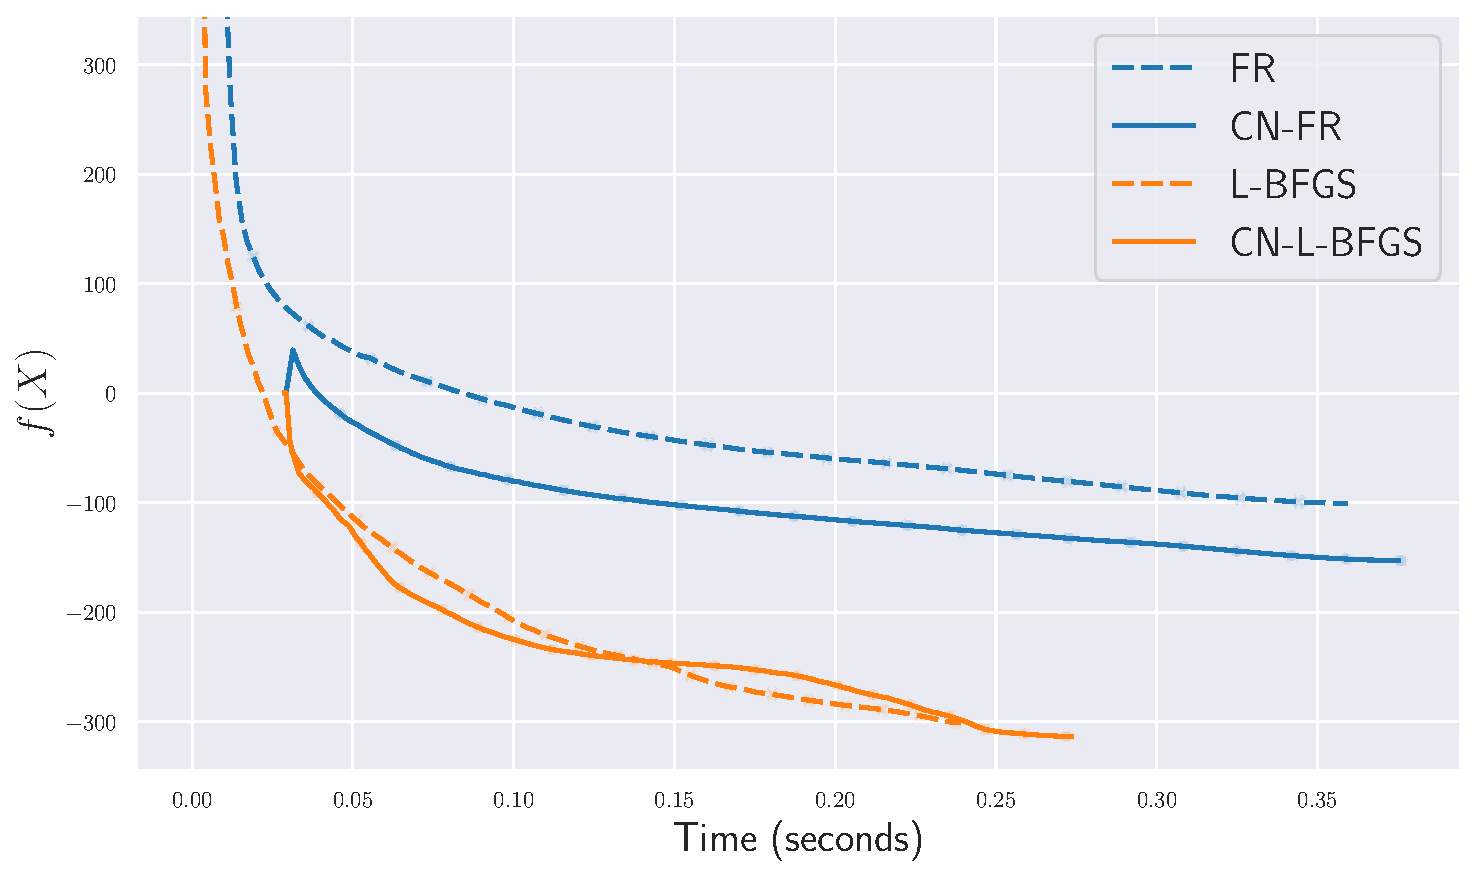
\includegraphics[width=0.55\columnwidth]{individual/plot/cycle300.pdf}} &
    \makecell{\small{\textsf{FR}}                                                                                                                        \\[-0.2em]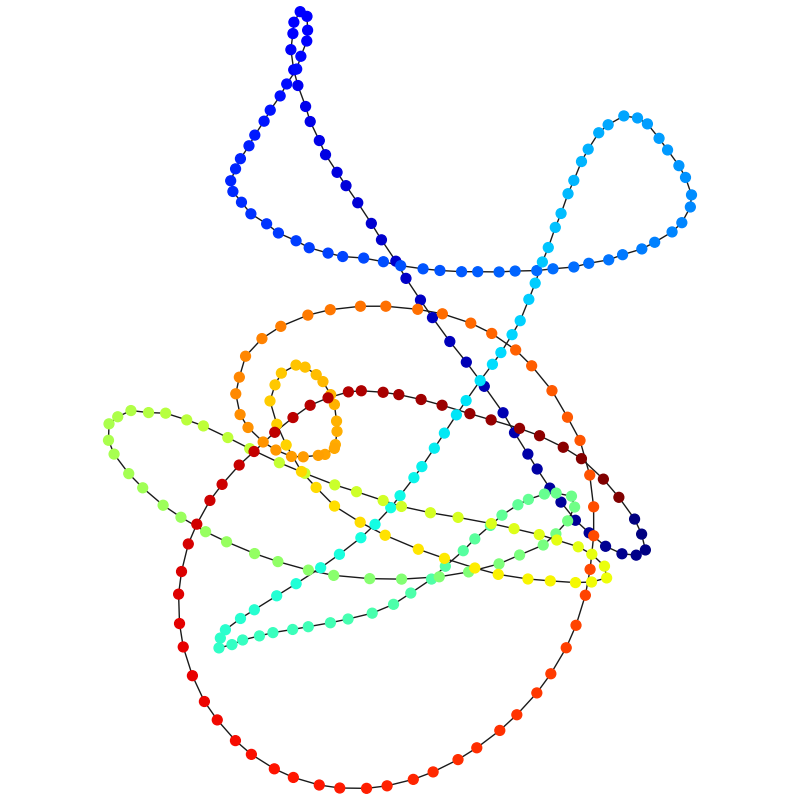
\includegraphics[width=0.27\columnwidth]{individual/vis/cycle300_FR.png}} &
    \makecell{\small{\textsf{L-BFGS}}                                                                                                                    \\[-0.2em]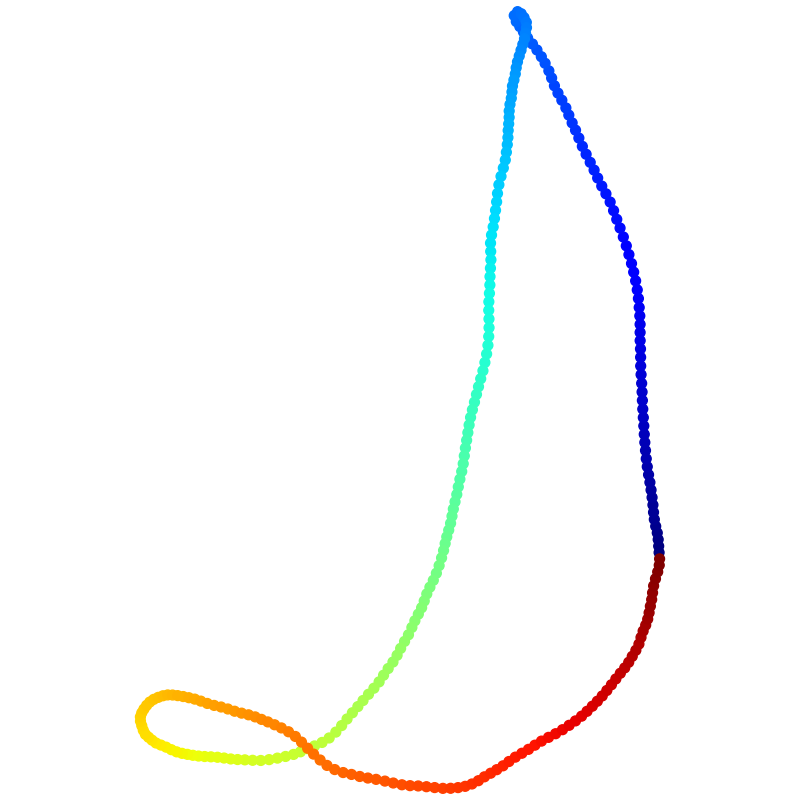
\includegraphics[width=0.27\columnwidth]{individual/vis/cycle300_L-BFGS.png}} &
    \makecell{\small{\textsf{CN-FR}}                                                                                                                     \\[-0.2em]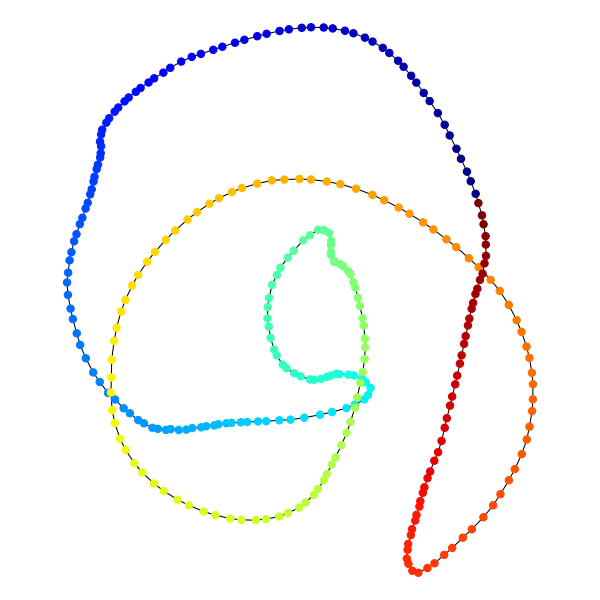
\includegraphics[width=0.27\columnwidth]{individual/vis/cycle300_CN-FR.png}} &
    \makecell{\small{\textsf{CN-L-BFGS}}                                                                                                                 \\[-0.2em]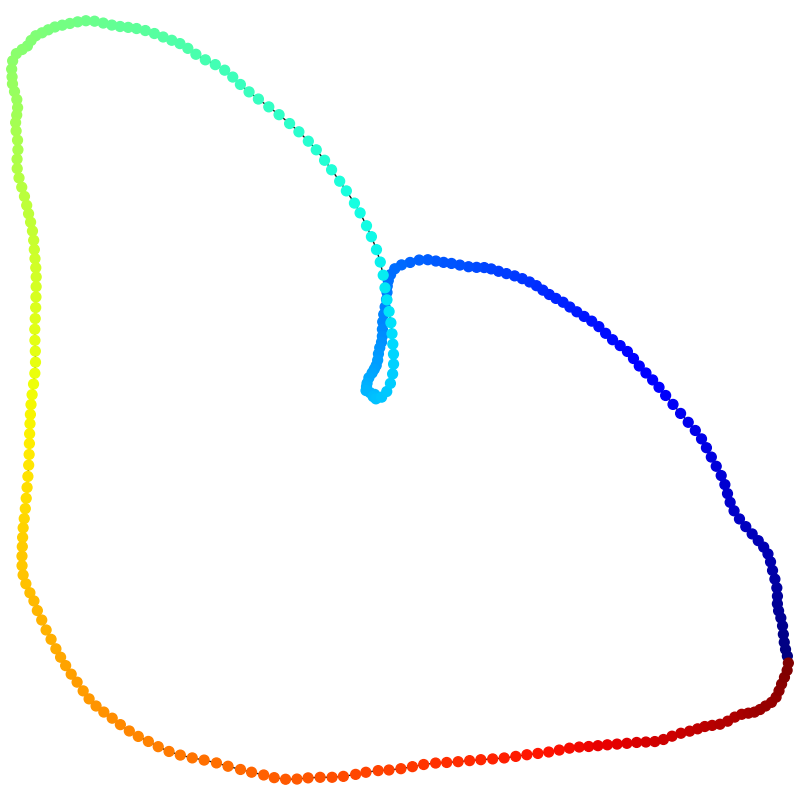
\includegraphics[width=0.27\columnwidth]{individual/vis/cycle300_CN-L-BFGS.png}} &
    \makecell{\small{\textsf{BEST}}                                                                                                                      \\[-0.2em]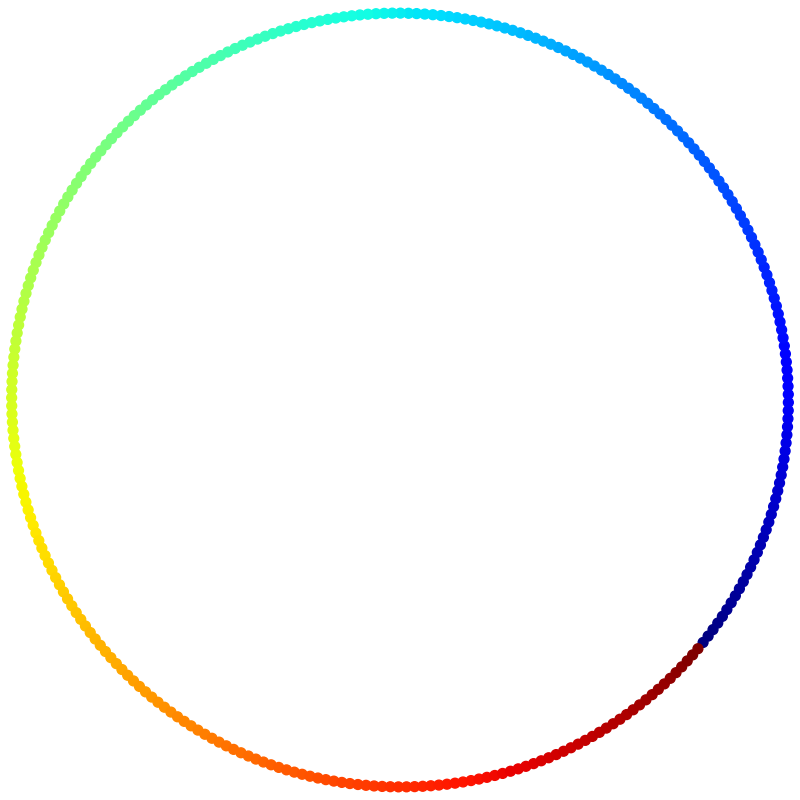
\includegraphics[width=0.27\columnwidth]{individual/vis/opt_cycle300.png}} \\

    \multicolumn{6}{c}{\textbf{\texttt{jagmesh1}} $(\abs{V}=936, \abs{E}=2664, \text{sparsity}=0.609\text{\%}) \quad Figures are at 50 iterations.$}     \\
    \raisebox{-.5\height}{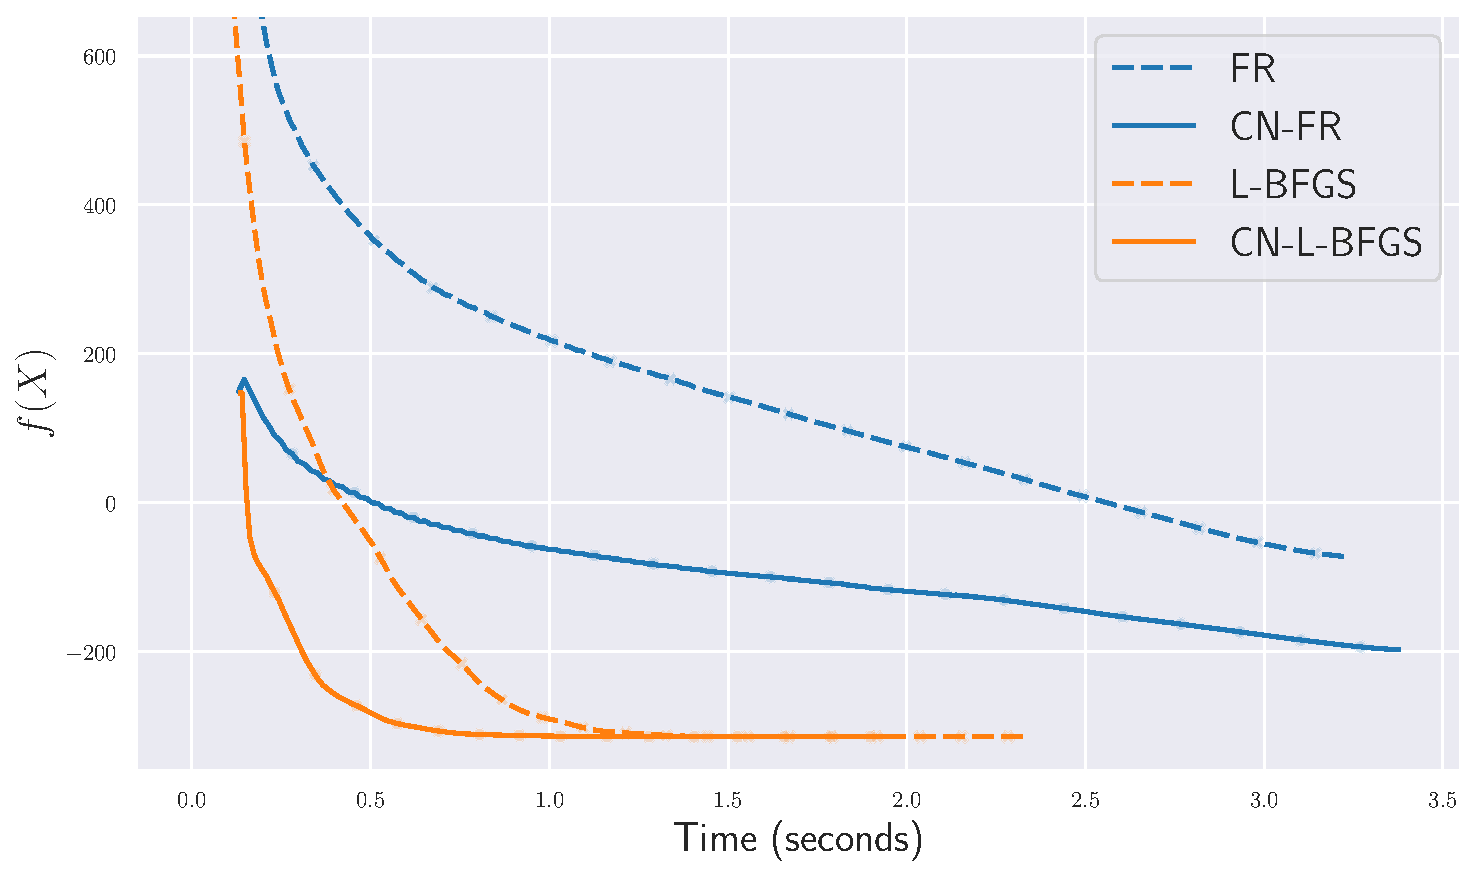
\includegraphics[width=0.55\columnwidth]{individual/plot/jagmesh1.pdf}} &
    \makecell{\small{\textsf{FR}}                                                                                                                        \\[-0.2em]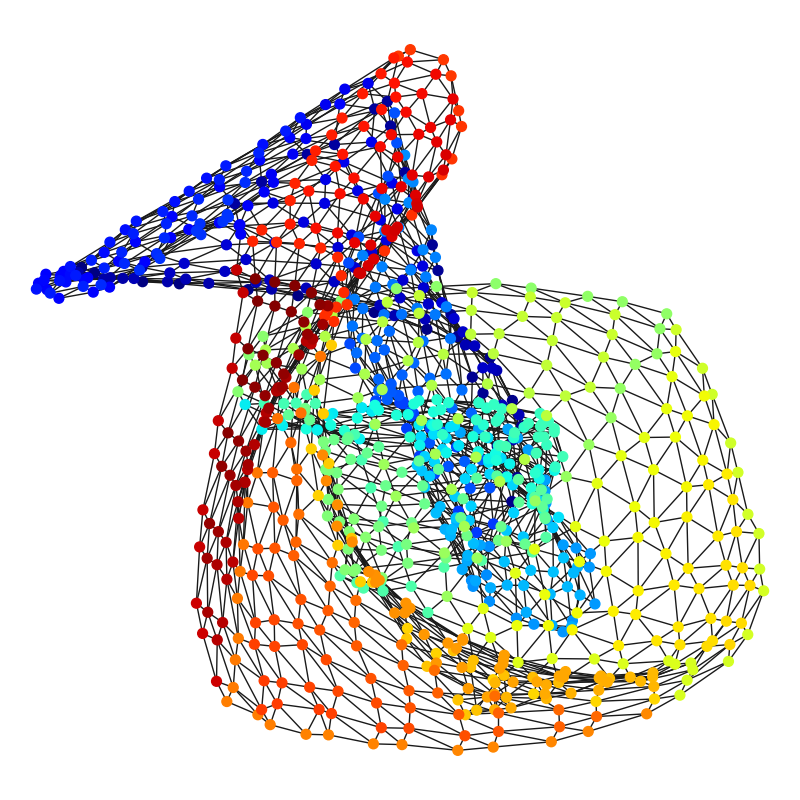
\includegraphics[width=0.27\columnwidth]{individual/vis/jagmesh1_FR.png}} &
    \makecell{\small{\textsf{L-BFGS}}                                                                                                                    \\[-0.2em]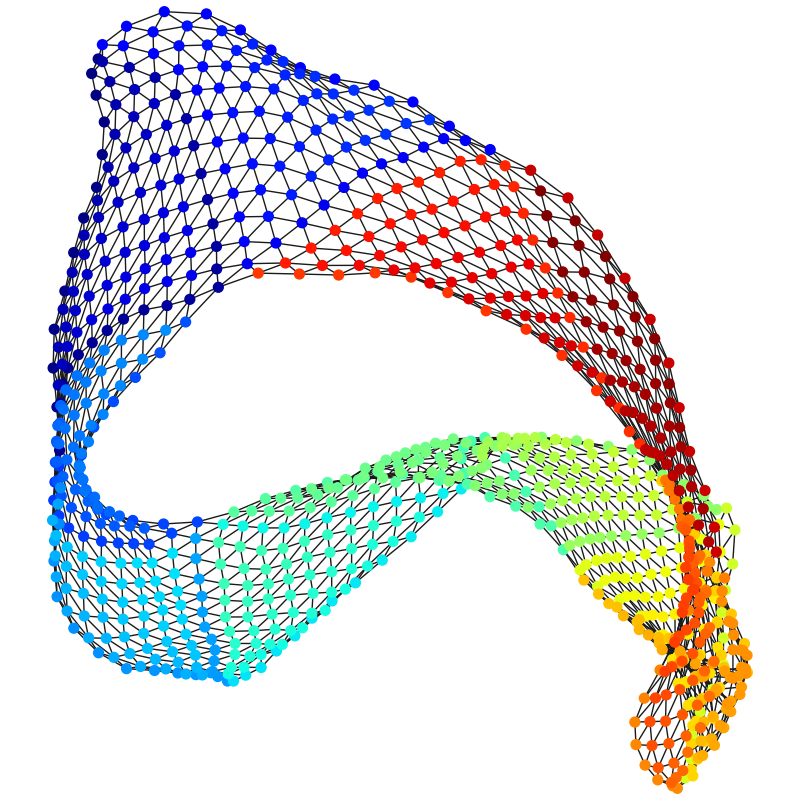
\includegraphics[width=0.27\columnwidth]{individual/vis/jagmesh1_L-BFGS.png}} &
    \makecell{\small{\textsf{CN-FR}}                                                                                                                     \\[-0.2em]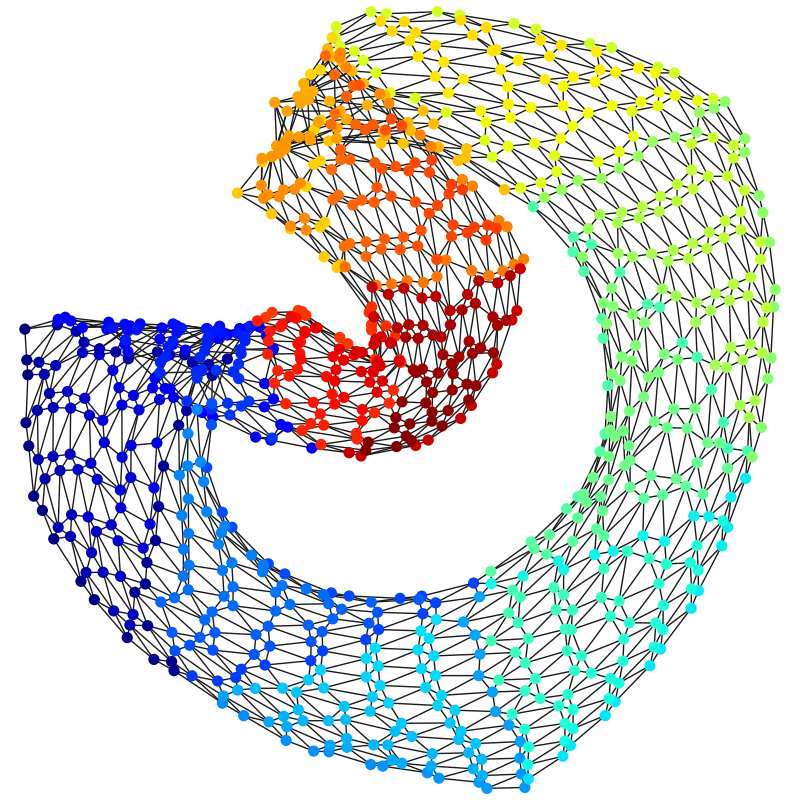
\includegraphics[width=0.27\columnwidth]{individual/vis/jagmesh1_CN-FR.png}} &
    \makecell{\small{\textsf{CN-L-BFGS}}                                                                                                                 \\[-0.2em]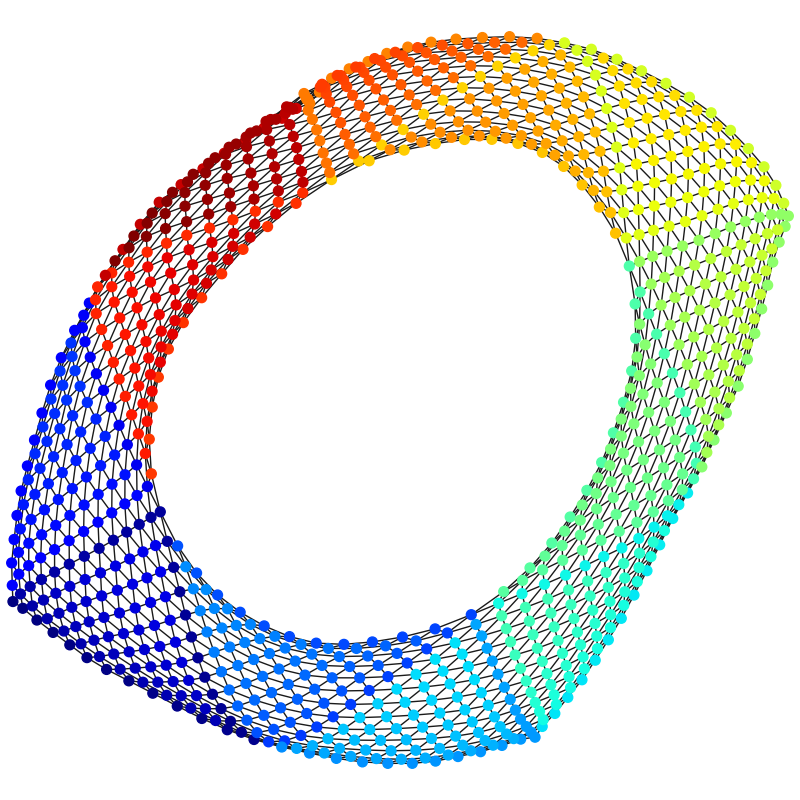
\includegraphics[width=0.27\columnwidth]{individual/vis/jagmesh1_CN-L-BFGS.png}} &
    \makecell{\small{\textsf{BEST}}                                                                                                                      \\[-0.2em]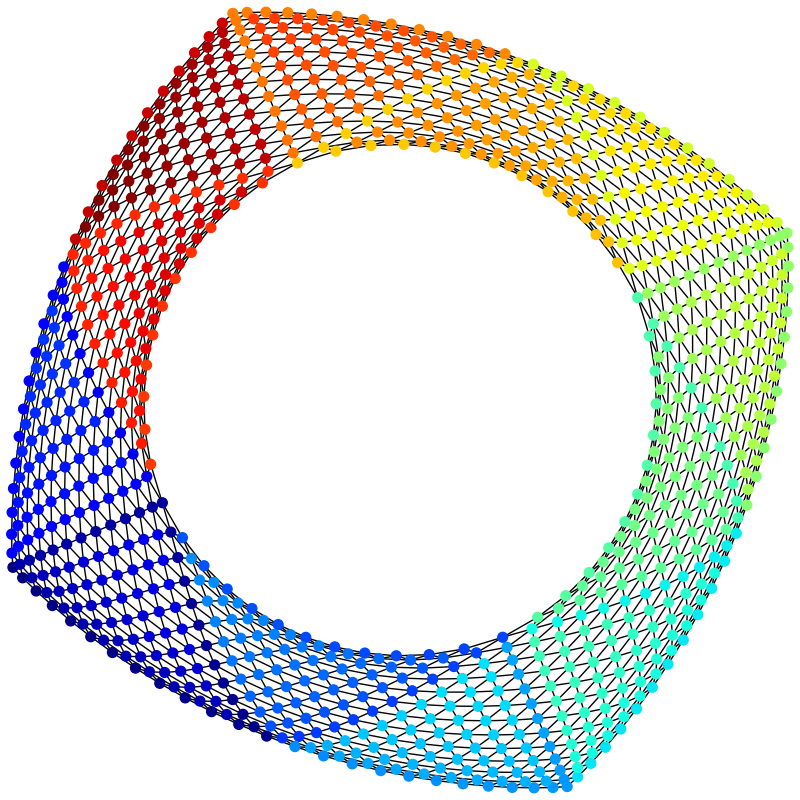
\includegraphics[width=0.27\columnwidth]{individual/vis/opt_jagmesh1.png}} \\

    \multicolumn{6}{c}{\textbf{\texttt{dwt\_1005}} $(\abs{V}=1005, \abs{E}=3808, \text{sparsity}=0.755\text{\%}) \quad Figures are at 100 iterations.$}  \\
    \raisebox{-.5\height}{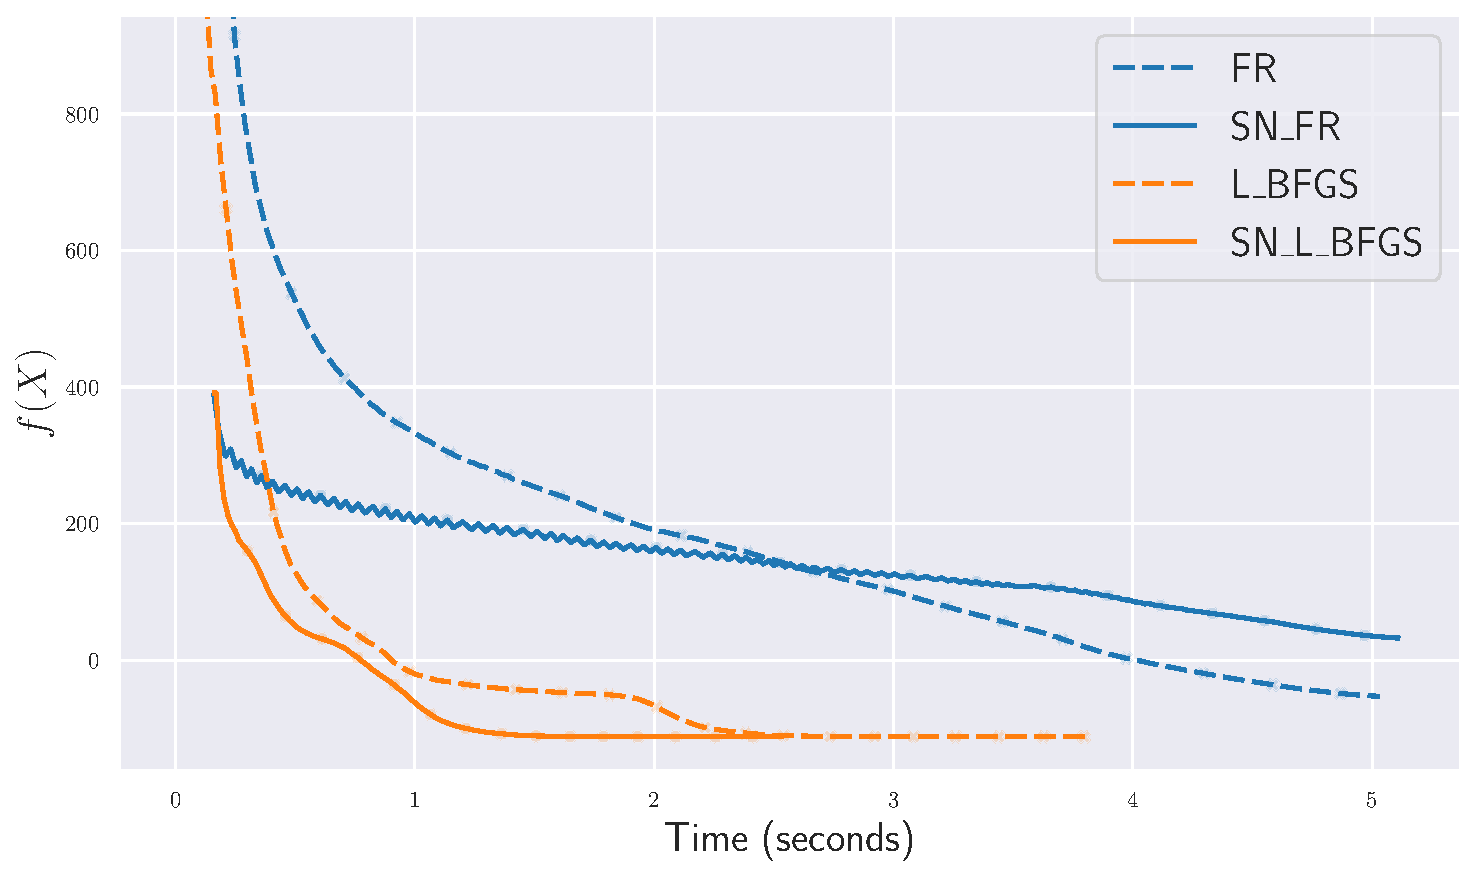
\includegraphics[width=0.55\columnwidth]{individual/plot/dwt_1005.pdf}} &
    \makecell{\small{\textsf{FR}}                                                                                                                        \\[-0.2em]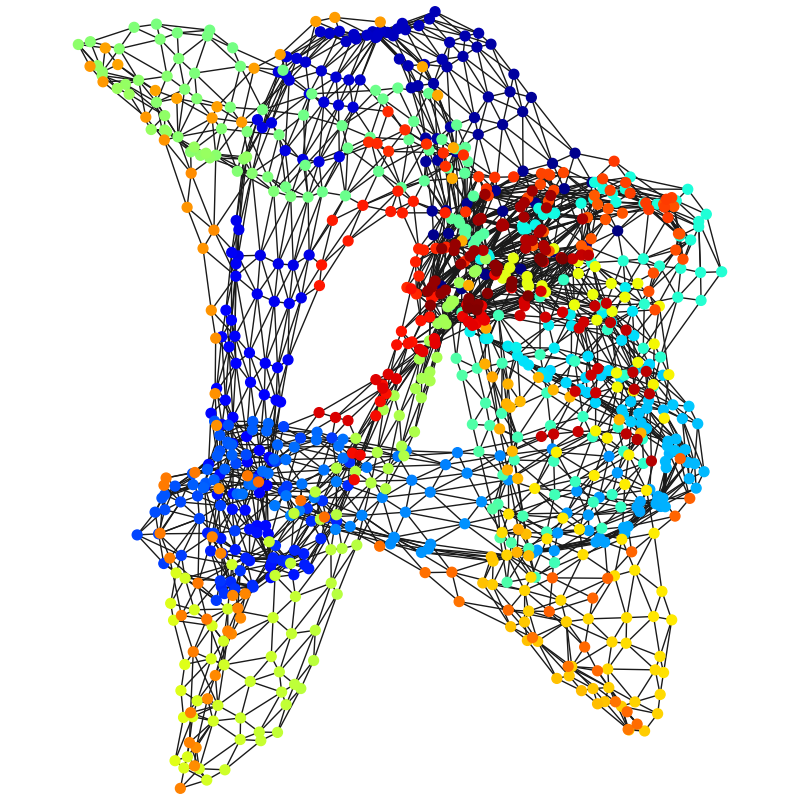
\includegraphics[width=0.27\columnwidth]{individual/vis/dwt_1005_FR.png}} &
    \makecell{\small{\textsf{L-BFGS}}                                                                                                                    \\[-0.2em]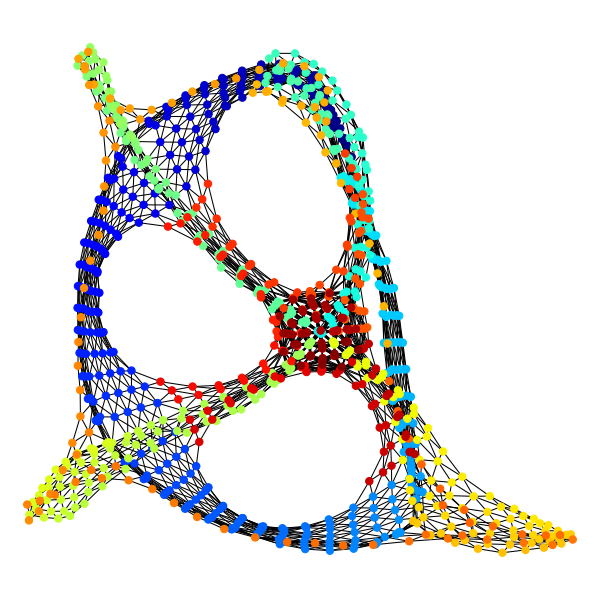
\includegraphics[width=0.27\columnwidth]{individual/vis/dwt_1005_L-BFGS.png}} &
    \makecell{\small{\textsf{CN-FR}}                                                                                                                     \\[-0.2em]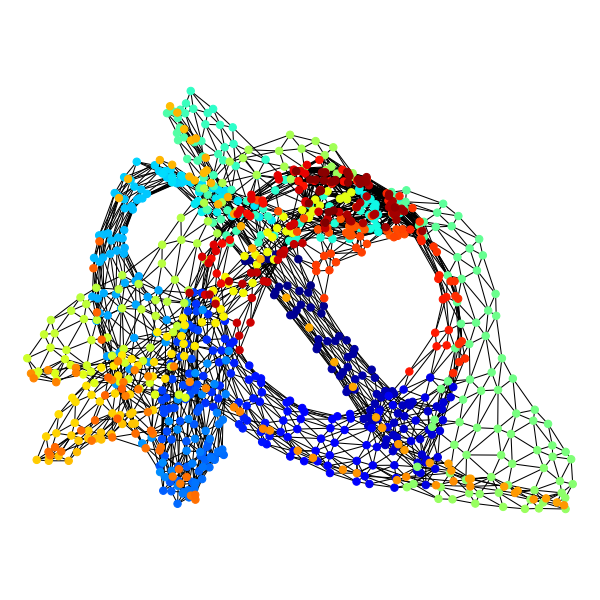
\includegraphics[width=0.27\columnwidth]{individual/vis/dwt_1005_CN-FR.png}} &
    \makecell{\small{\textsf{CN-L-BFGS}}                                                                                                                 \\[-0.2em]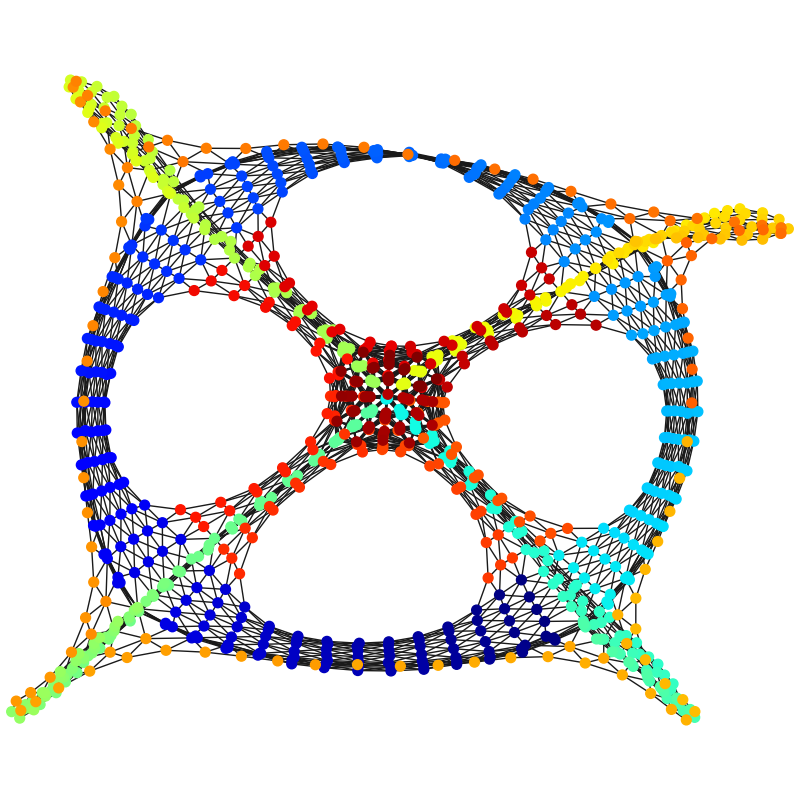
\includegraphics[width=0.27\columnwidth]{individual/vis/dwt_1005_CN-L-BFGS.png}} &
    \makecell{\small{\textsf{BEST}}                                                                                                                      \\[-0.2em]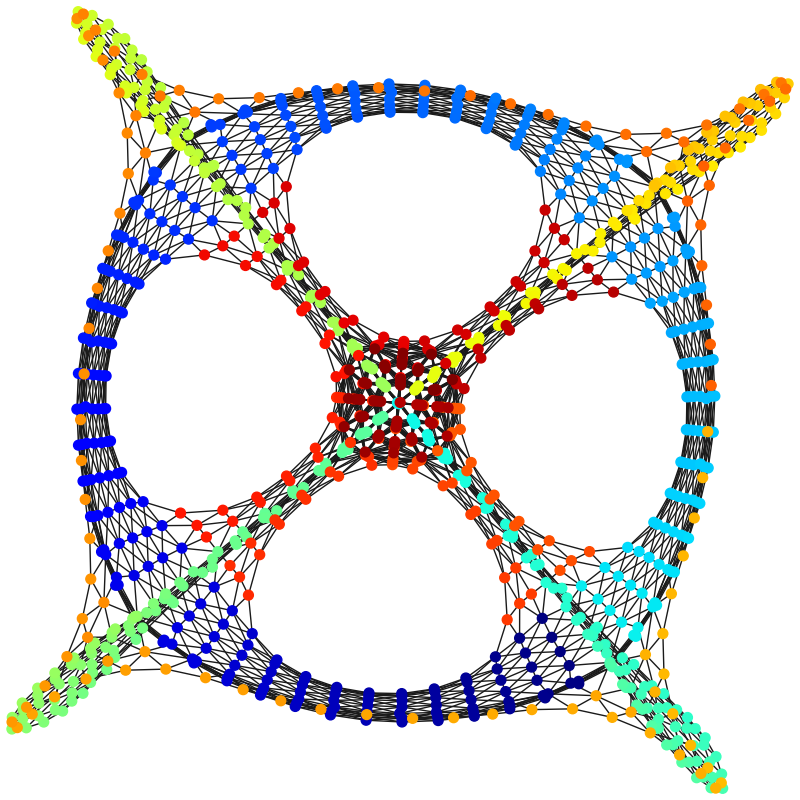
\includegraphics[width=0.27\columnwidth]{individual/vis/opt_dwt_1005.png}} \\

    \multicolumn{6}{c}{\textbf{\texttt{btree9}} $(\abs{V}=1023, \abs{E}=1022, \text{sparsity}=0.196\text{\%}) \quad Figures are at 150 iterations.$}     \\
    \raisebox{-.5\height}{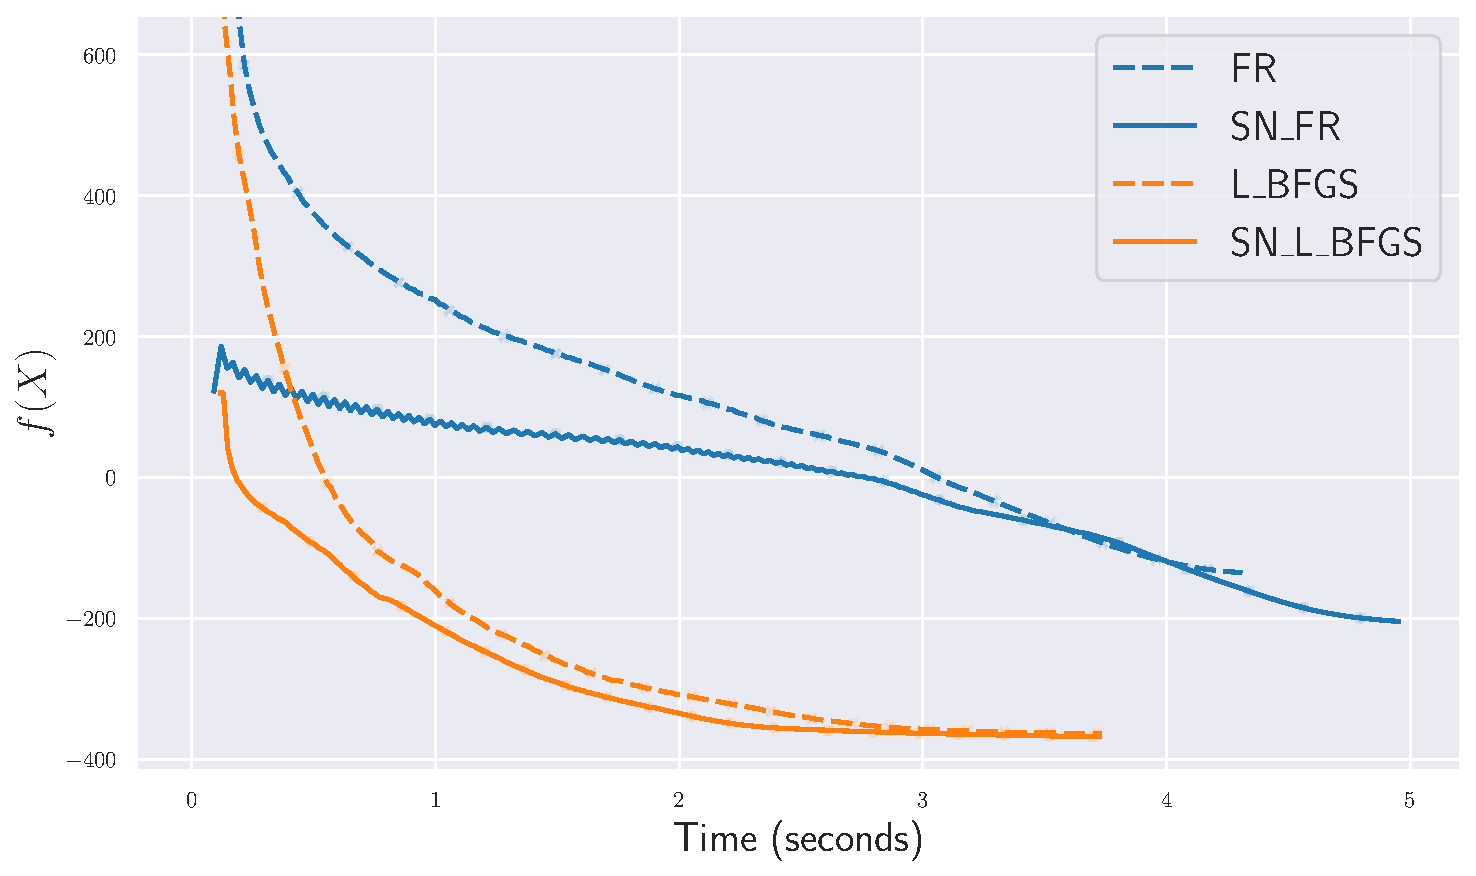
\includegraphics[width=0.55\columnwidth]{individual/plot/btree9.pdf}}   &
    \makecell{\small{\textsf{FR}}                                                                                                                        \\[-0.2em]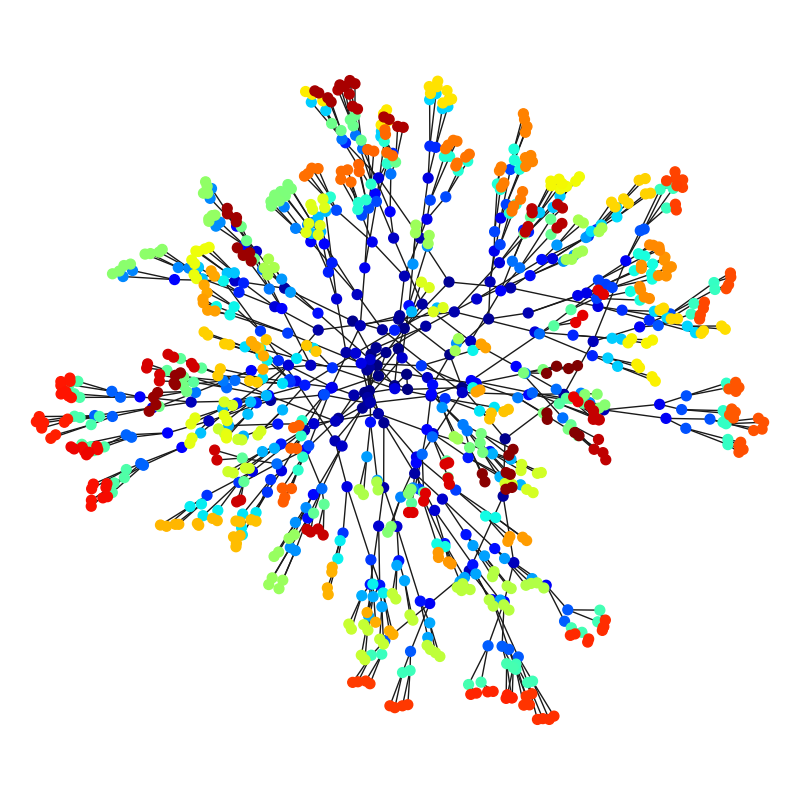
\includegraphics[width=0.27\columnwidth]{individual/vis/btree9_FR.png}} &
    \makecell{\small{\textsf{L-BFGS}}                                                                                                                    \\[-0.2em]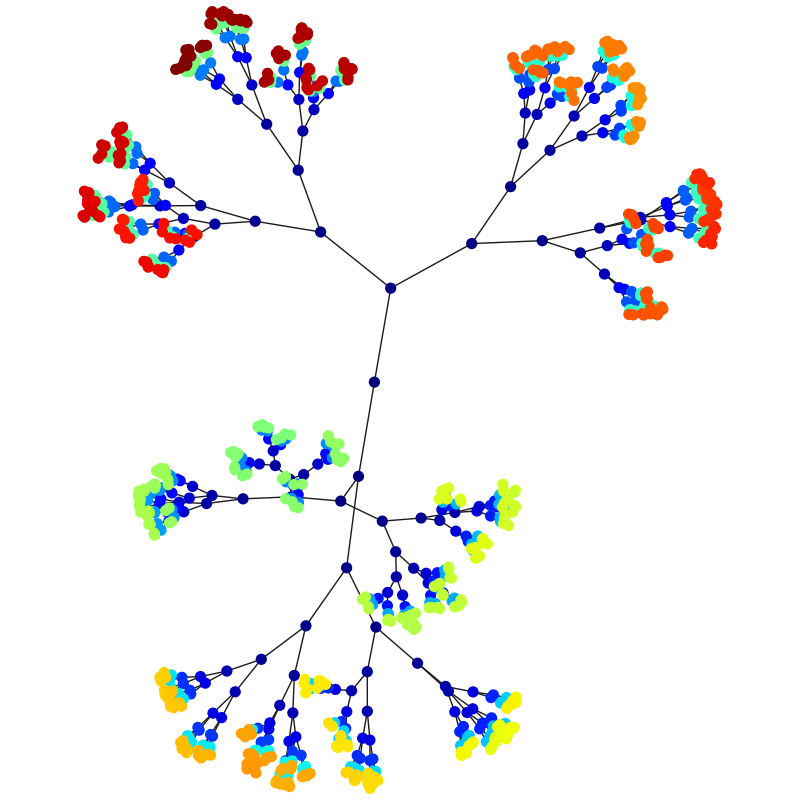
\includegraphics[width=0.27\columnwidth]{individual/vis/btree9_L-BFGS.png}} &
    \makecell{\small{\textsf{CN-FR}}                                                                                                                     \\[-0.2em]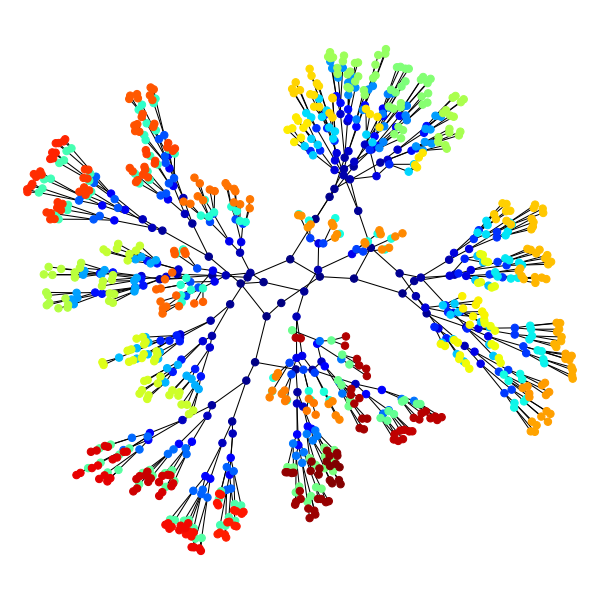
\includegraphics[width=0.27\columnwidth]{individual/vis/btree9_CN-FR.png}} &
    \makecell{\small{\textsf{CN-L-BFGS}}                                                                                                                 \\[-0.2em]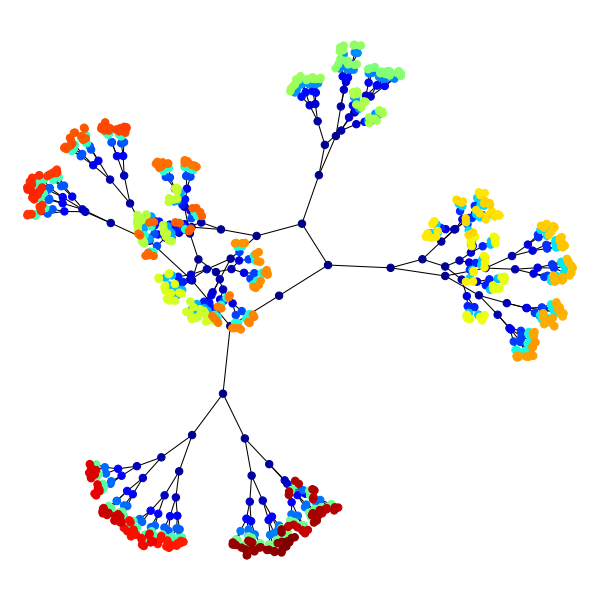
\includegraphics[width=0.27\columnwidth]{individual/vis/btree9_CN-L-BFGS.png}} &
    \makecell{\small{\textsf{BEST}}                                                                                                                      \\[-0.2em]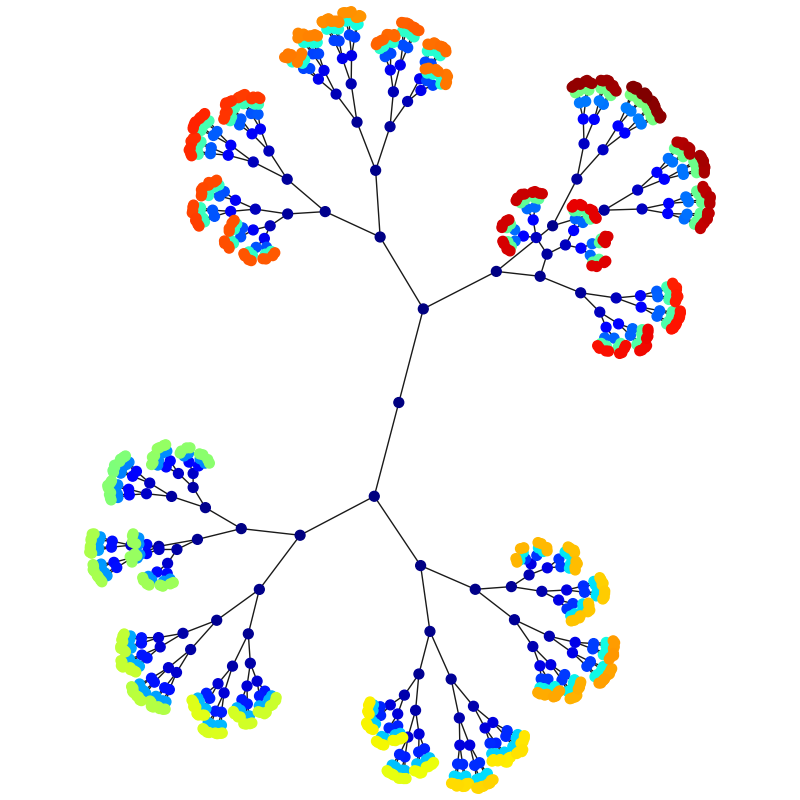
\includegraphics[width=0.27\columnwidth]{individual/vis/opt_btree9.png}} \\

    \multicolumn{6}{c}{\textbf{\texttt{1138\_bus}} $(\abs{V}=1138, \abs{E}=1458, \text{sparsity}=0.225\text{\%}) \quad Figures are at 150 iterations.$}  \\
    \raisebox{-.5\height}{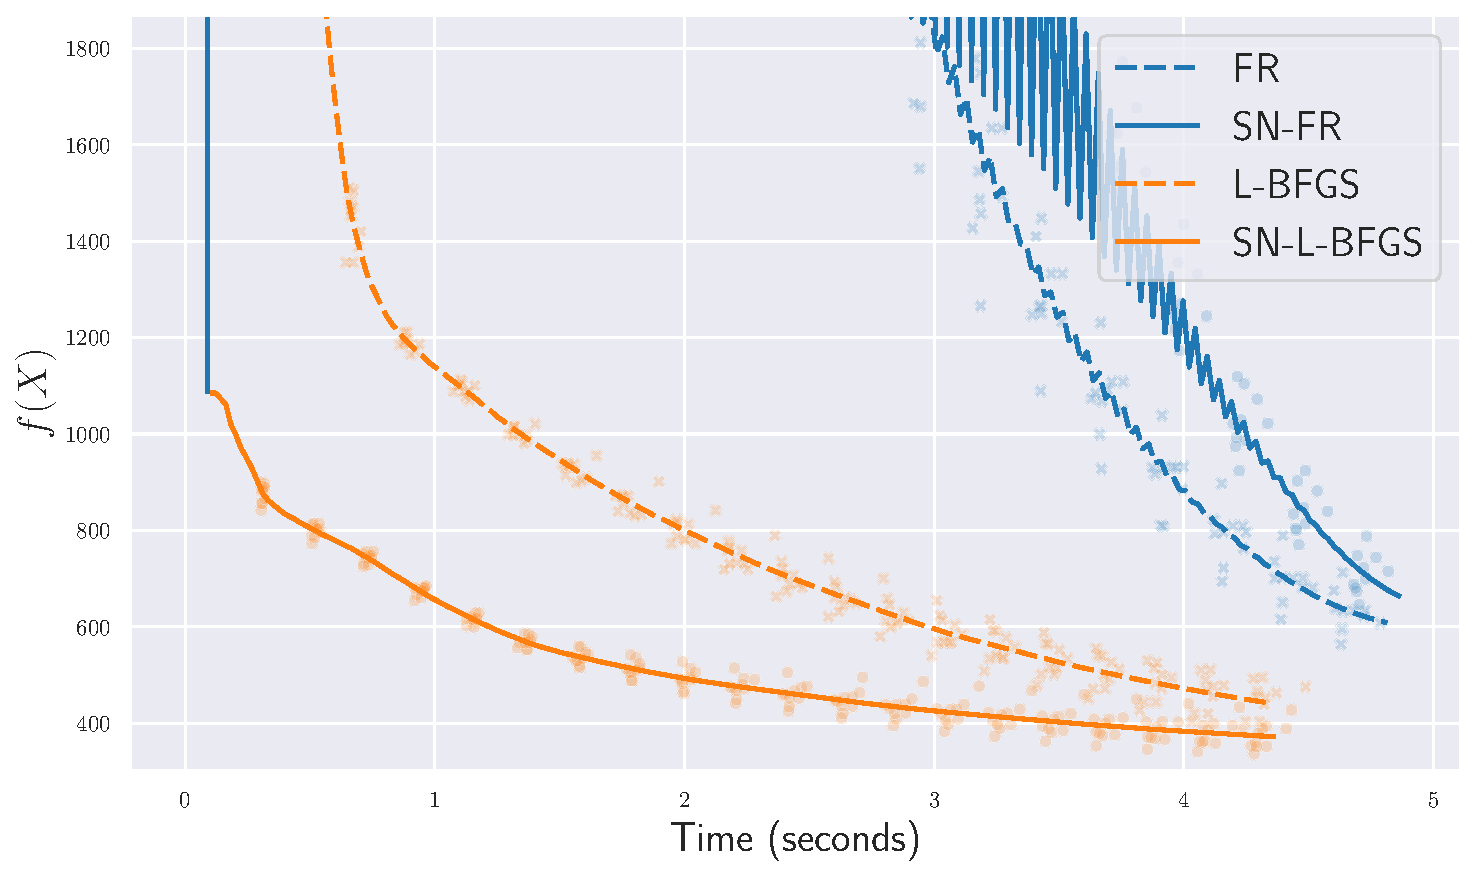
\includegraphics[width=0.55\columnwidth]{individual/plot/1138_bus.pdf}} &
    \makecell{\small{\textsf{FR}}                                                                                                                        \\[-0.2em]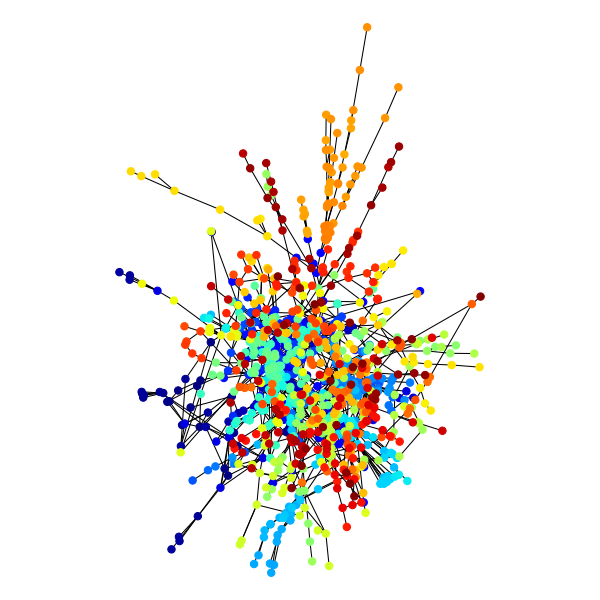
\includegraphics[width=0.27\columnwidth]{individual/vis/1138_bus_FR.png}} &
    \makecell{\small{\textsf{L-BFGS}}                                                                                                                    \\[-0.2em]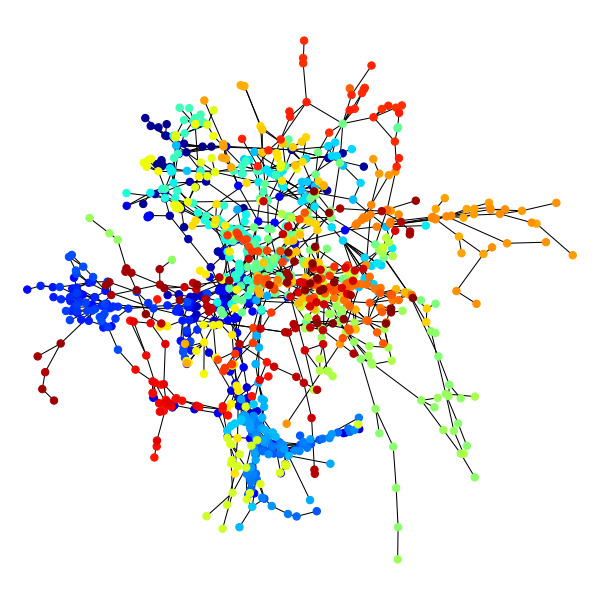
\includegraphics[width=0.27\columnwidth]{individual/vis/1138_bus_L-BFGS.png}} &
    \makecell{\small{\textsf{CN-FR}}                                                                                                                     \\[-0.2em]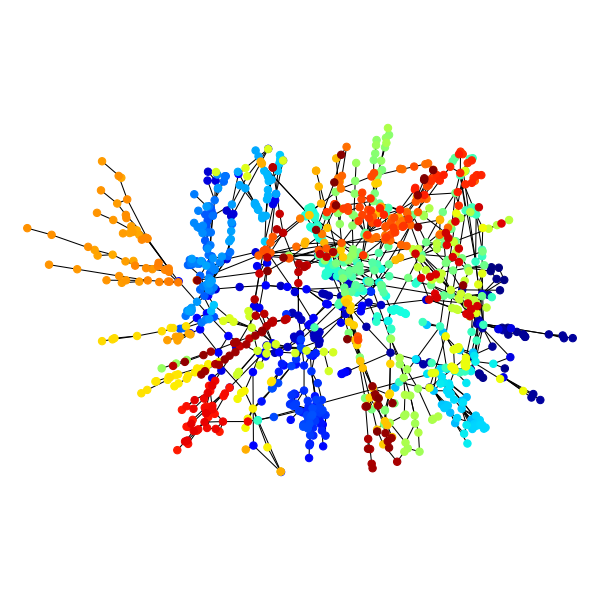
\includegraphics[width=0.27\columnwidth]{individual/vis/1138_bus_CN-FR.png}} &
    \makecell{\small{\textsf{CN-L-BFGS}}                                                                                                                 \\[-0.2em]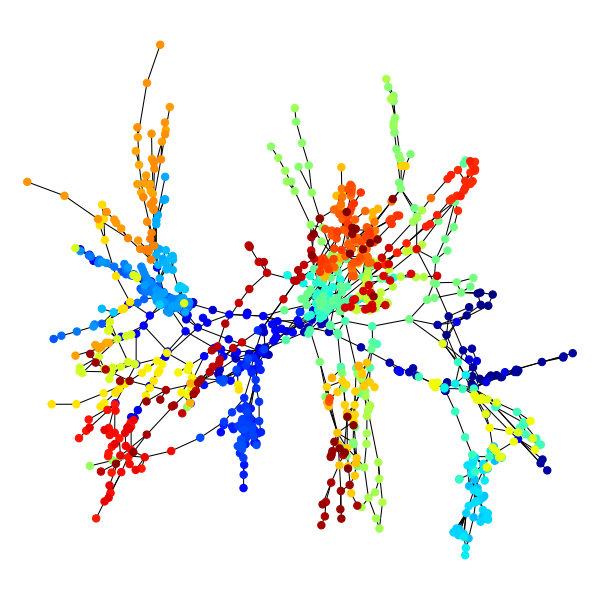
\includegraphics[width=0.27\columnwidth]{individual/vis/1138_bus_CN-L-BFGS.png}} &
    \makecell{\small{\textsf{BEST}}                                                                                                                      \\[-0.2em]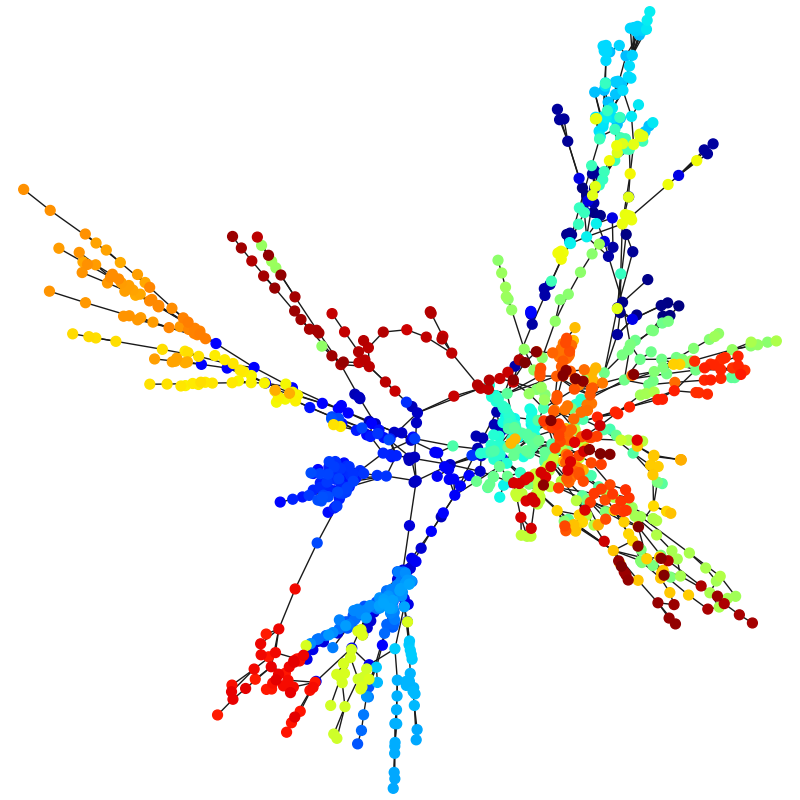
\includegraphics[width=0.27\columnwidth]{individual/vis/opt_1138_bus.png}} \\

    \multicolumn{6}{c}{\textbf{\texttt{dwt\_2680}} $(\abs{V}=2680, \abs{E}=11173, \text{sparsity}=0.311\text{\%}) \quad Figures are at 150 iterations.$} \\
    \raisebox{-.5\height}{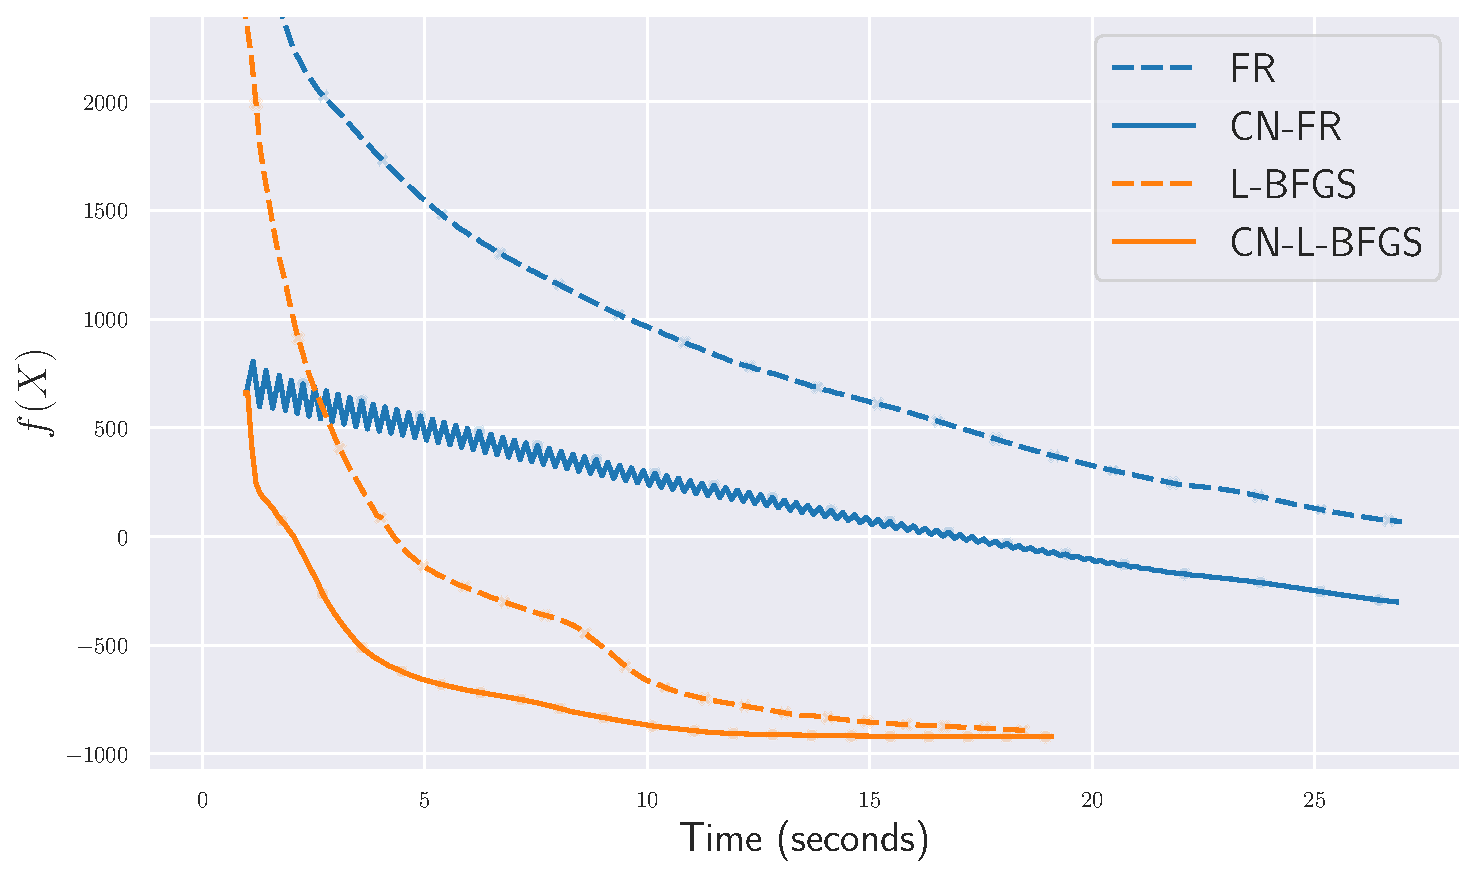
\includegraphics[width=0.55\columnwidth]{individual/plot/dwt_2680.pdf}} &
    \makecell{\small{\textsf{FR}}                                                                                                                        \\[-0.2em]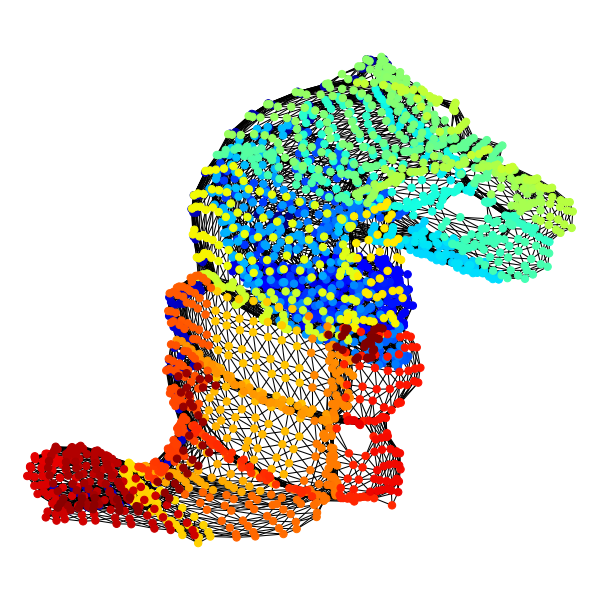
\includegraphics[width=0.27\columnwidth]{individual/vis/dwt_2680_FR.png}} &
    \makecell{\small{\textsf{L-BFGS}}                                                                                                                    \\[-0.2em]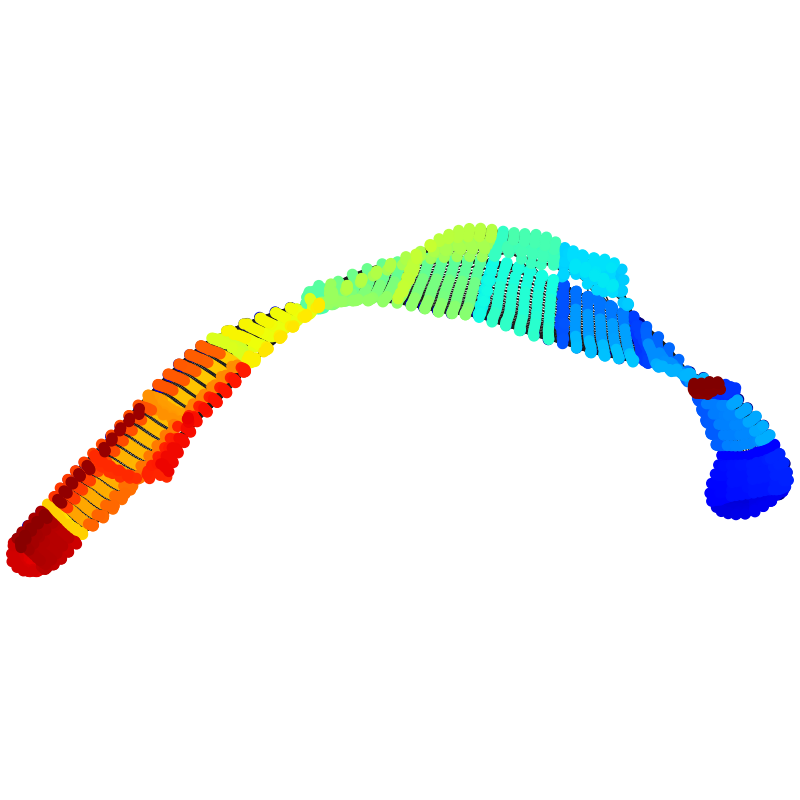
\includegraphics[width=0.27\columnwidth]{individual/vis/dwt_2680_L-BFGS.png}} &
    \makecell{\small{\textsf{CN-FR}}                                                                                                                     \\[-0.2em]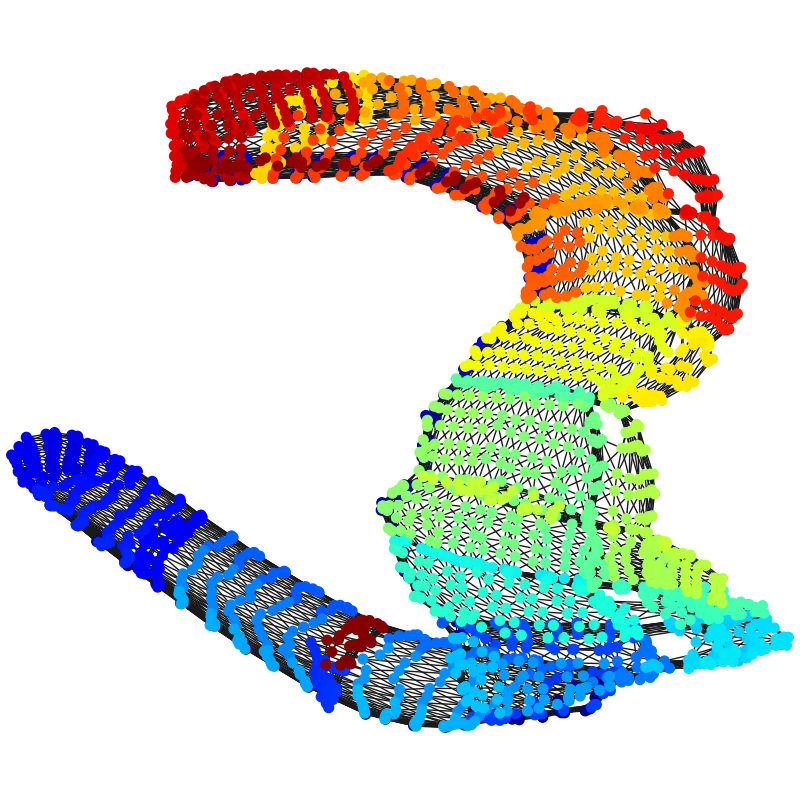
\includegraphics[width=0.27\columnwidth]{individual/vis/dwt_2680_CN-FR.png}} &
    \makecell{\small{\textsf{CN-L-BFGS}}                                                                                                                 \\[-0.2em]\includegraphics[width=0.27\columnwidth]{individual/vis/dwt_2680_CN-L-BFGS.png}} &
    \makecell{\small{\textsf{BEST}}                                                                                                                      \\[-0.2em]\includegraphics[width=0.27\columnwidth]{individual/vis/opt_dwt_2680.png}} \\

    \multicolumn{6}{c}{\textbf{\texttt{3elt}} $(\abs{V}=4720, \abs{E}=13722, \text{sparsity}=0.123\text{\%}) \quad Figures are at 150 iterations.$}      \\
    \raisebox{-.5\height}{\includegraphics[width=0.55\columnwidth]{individual/plot/3elt.pdf}}     &
    \makecell{\small{\textsf{FR}}                                                                                                                        \\[-0.2em]\includegraphics[width=0.27\columnwidth]{individual/vis/3elt_FR.png}} &
    \makecell{\small{\textsf{L-BFGS}}                                                                                                                    \\[-0.2em]\includegraphics[width=0.27\columnwidth]{individual/vis/3elt_L-BFGS.png}} &
    \makecell{\small{\textsf{CN-FR}}                                                                                                                     \\[-0.2em]\includegraphics[width=0.27\columnwidth]{individual/vis/3elt_CN-FR.png}} &
    \makecell{\small{\textsf{CN-L-BFGS}}                                                                                                                 \\[-0.2em]\includegraphics[width=0.27\columnwidth]{individual/vis/3elt_CN-L-BFGS.png}} &
    \makecell{\small{\textsf{BEST}}                                                                                                                      \\[-0.2em]\includegraphics[width=0.27\columnwidth]{individual/vis/opt_3elt.png}} \\
  \end{tabular}
  \caption{Numerical experiment results for various graphs.  Please refer Sec.~\ref{ssec:exprDetail} for details.}
  \label{fig:individual}
\end{figure*}

We also conducted a detailed experiment to investigate the behavior of the proposed algorithm in detail. The result is shown in Fig.~\ref{fig:individual}.

The experiment details are as follows.
As parameters, we used $N_\mathrm{iter}^\mathsf{FR} = N_\mathrm{iter}^\mathsf{L-BFGS} = 200$ as the maximum number of iterations.
We tested with 7 graphs: \texttt{cycle300}, \texttt{jagmesh1}, \texttt{dwt\_1005}, \texttt{btree9}, \texttt{1138\_bus}, \texttt{dwt\_2680}, and \texttt{3elt}. \texttt{cycle300} is a cycle graph with 300 vertices, and btree9 is a perfect binary tree with $2^{9+1}-1=1023$ vertices. Other graphs are from Sparse Matrix Collection~\cite{davis2011university}, and these choices are based on the experiments conducted in Ref.~\cite{8419285}. Thus, although all the graphs are quite sparse so that $\abs{E} / (\abs{V}(V-1)/2)$ is less than 1\%, this is not an arbitrary choice. The important graphs often have such a sparsity.

We first explain what Fig.~\ref{fig:individual} represents.
The plots on the left illustrate the objective function values $f(X)$ on the vertical axis versus execution time on the horizontal axis, using 10 trials for each algorithm.
Faint crosses represent the results of non-\textsf{CN} algorithms, while faint circles represent the results of \textsf{CN} algorithms, plotted every 10 iterations for each trial.
The solid and dashed lines represent the average of these values across the 10 trials for each algorithm.
If one of the trials terminated before reaching $N_\mathrm{iter}^\mathsf{FR}$ or $N_\mathrm{iter}^\mathsf{L-BFGS}$ iterations, the line was plotted up to the minimum trial count achieved across all trials.
Each trial was conducted with a different seed, meaning that even deterministic algorithms, such as
\textsf{FR} or \textsf{L-BFGS}, converged to different local optima due to variations in the initial random placement.
The graphs on the right illustrates the placement at the 150th iteration (or the final iteration if it concluded before then) for each algorithm with the seed 0.

The observations and implications of Fig.~\ref{fig:individual} are as follows.
First, the solid plots for \textsf{CN} generally demonstrates superior performance compared to non-\textsf{CN}, validating the efficacy of the proposed method.
Some exception of the superiority arise with \textsf{FR}, which exhibits oscillations in the plot, likely due to excessive step sizes leading to overshooting.
Although we refrained from altering \textsf{FR} for fairness, adjusting the step size could enable the proposed method to achieve its intended performance.
In fact, the initial $f(X)$ of \textsf{CN-FR} is clearly small enough compared to the objective function values produced by \textsf{FR} alone, suggesting that the proposed method is yielding a good initial placement.
Additionally, the visualization results support the effectiveness of the proposed initial placement. In most cases, placements obtained with \textsf{CN} better represent the intended geometric arrangement compared to non-\textsf{CN} placements.

As a side note, regardless of \textsf{CN} or non-\textsf{CN}, the algorithms using \textsf{L-BFGS} consistently outperforms those using \textsf{FR}.
This finding is consistent with prior research~\cite{6183577}, though, regrettably, this technique remains relatively unknown in the field of graph drawing.
One of the aims of our paper is to further emphasize and popularize the use of \textsf{L-BFGS} in graph drawing, and these results provide a strong basis for this argument.

\section{Challenges of the Coordinate Newton Direction}\label{sec:challenges}

Here, we explain the rationale for why we took a roundabout approach to optimize Prob.~\eqref{eq:fr}.
As we have explained, we first transformed it into a discrete optimization problem, Prob.~\eqref{eq:frApprox3}, and then optimized it using the coordinate Newton direction. However, is it possible to directly leverage the coordinate Newton direction to optimize Prob.~\eqref{eq:fr}?
We think the answer is no, and in this section, we explain the reasons behind this conclusion.

The important point is that these issues do not necessarily preclude the possibility of achieving global optimization with the coordinate Newton direction.
Rather, we hope that an accurate understanding of these challenges will lead us to develop better optimization methods in the future.

\subsection{Possible Approach with Coordinate Newton Direction}\label{ssec:possibleApproach}

In this subsection, we explain a possible approach to optimize Prob.~\eqref{eq:fr} using the coordinate Newton direction.
As mentioned, our approach resembles to the RSN method, one of the subspace methods, and RSN and its variant have been proposed in the context of continuous optimization~\cite{NEURIPS2019_bc6dc48b,
  fujiRandomizedSubspaceRegularized2022,
  cartisRandomisedSubspaceMethods2022,
  nozawaRandomizedSubspaceGradient2023,
  higuchiFastConvergenceSecondOrder2024}.

We take the following algorithm as a direct application of the subspace methods to the FR layout; Namely, we randomly select a vertex $v_i$, apply Newton's method or its regularized variant to $f_i$ using the gradient in Eq.~\eqref{eq:gradientFi} and its Hessian:
\begin{gather*}
  \nabla^2 f_i(x_i) = \sum_{j \neq i} \left(\frac{w_{i,j}\norm{x_i - x_j}}{k} - \frac{k^2}{\norm{x_i - x_j}^2}\right) I_d + \\
  \sum_{j \neq i} \left(\frac{w_{i,j}}{k \norm{x_i - x_j}} + \frac{2k^2}{\norm{x_i - x_j}^4}\right) (x_i - x_j)(x_i - x_j)^\top.
\end{gather*}
Then, we update the position of vertex $v_i$, and repeat this process until convergence.
However, this approach fails to work effectively in practice.
In the following, we explain the reasons behind this difficulty.

\subsection{Inaccuracy of quadratic approximation}\label{ssec:inaccuracy}

\begin{figure}[t]
  \centering
  \includegraphics[height=2.2cm]{whyRSNfail/whyRSNfail.pdf}
  \caption{
    The inaccurate quadratic approximation.
    Assume that the optimal placement of the graph is as shown on the left.
    For the red vertex on the right graph, its Newton direction is the red arrow, which is apparently a bad direction.
  }
  \label{fig:whyRSNfail}
\end{figure}

This subsection discusses the inaccuracy of quadratic approximation used in the Newton's method, particularly a specific issue arises when restricting the optimization to a subspace.

When we apply the Newton's method to a randomly selected vertex $v_i$, we approximate the energy function $f_i$ as a quadratic function $\overline{f}_i$ at $x_i$.
If this approximated function is convex, then the Newton's method update $v_i$ to the optimal solution of the approximated function.
Otherwise, by adding regularization terms, such as the cubic regularization~\cite{nesterovCubicRegularizationNewton2006}, we can update $v_i$ to a descent direction of $\overline{f}_i$.

Nevertheless, the update of $x_i$, which locally improves $\overline{f}_i$, does not necessarily improves the overall energy function $f$.

We show an example of this issue in Fig.~\ref{fig:whyRSNfail}.
Let a graph $G$ be as shown in the left (optimal), where $k$ and all positive edge weights $w_{i,j}$ are set to 1.
In a successful case such as in the middle (success), the subspace method works effectively, since the Newton direction defined on $f_i$ (blue arrow) leads to the improvement of the overall energy function $f$.

However, in the situation depicted on the right (failure), the Newton direction for $x_1$ (red arrow) is apparently a bad direction, leading to a significant deviation from the global optimal solution as it is.
The points of $G$ are set as
\begin{equation*}
  X = \begin{pmatrix}
    0 & -1 & -0.85  & -0.85  & 1 \\
    0 & 0  & +0.155 & -0.155 & 0
  \end{pmatrix},
\end{equation*}
and the Hessian $\nabla^2 f_1(x_1)$ is approximately
\begin{equation*}
  \begin{pmatrix}
    1.841 & 0     \\
    0     & 1.159
  \end{pmatrix},
\end{equation*}
which is positive definite and not ill-conditioned.
Despite of such a good property of the Hessian, the Newton direction for $x_1$ (red arrow) is a bad direction, since the repulsive force between $x_1$ and $x_2,x_3$ are too strong to diverge from the global optimal solution.
This kind of illness cannot be resolved by just modifying the Newton's method we use for $f_i$, and it is a inherent problem of the subspace method.

\subsection{Ignorance of other vertex movements}\label{ssec:ignorance}

\begin{figure}[t]
  \centering
  \includegraphics[height=2.2cm]{whyRSNfail2/whyRSNfail2.pdf}
  \caption{
    The ignorance of other vertex movements. Assume that the blue arrows show the forces to the vertices and the optimal movements in this situation. Nevertheless, the red vertex will only move a little by the subspace method.
  }
  \label{fig:whyRSNfail2}
\end{figure}

This subsection discusses another issue of the subspace method, which is the ignorance of other vertex movements when optimizing each vertex individually.
When optimizing for a vertex $v_i$, the subspace method treat all other vertices $v_j (j \neq i)$ as fixed. However, both the FR algorithm and the L-BFGS algorithm do not, which represents a significant difference.

This is illustrated in Figure~\ref{fig:whyRSNfail2}.
Consider a subset of vertices in a mesh-like structure $G$, all vertices receive forces to the blue arrow directions and can minimize $f$ by moving in that direction.
In this setting, both the FR algorithm and the L-BFGS algorithm progress the optimization without issue.
On the other hand, if we attempt to optimize only for the red vertex in the right graph, heavily influenced by its directly connected neighbors, $v_0$ barely moves.
As a result, the overall optimization barely advances, in contrast to the alignment of the blue arrows.
The same problem occurs for other vertices.

In this way, ignoring the direction of forces on other vertices, or more precisely, neglecting the values of $\pdv{f}{x_i}{x_j}$, is a major shortcoming of the subspace method.

\subsection{Rationale for the Proposed Method}\label{ssec:rationale}

As explained, we suspect that, while the subspace method is effective for reducing the ``twist'' in a rough sense, it is not suitable for optimizing the overall placement.

However, by converting the problem as stated in Section~\ref{ssec:reduction}, we can take this ignored interaction into account to some extent.
The advantage of Prob.~\eqref{eq:frApprox3} is that not only reduction of the computational complexity from $\order{\abs{V}^2}$ to $\order{\abs{E}}$, but also allowing us to more easily take account for vertex interactions and prevent them from becoming too close to each other, since the mapping $\pi$ is injection.
Thus, making the problem discrete brings the acceleration of each iteration as well as the high quality of the updated solution.

The important point is that, combined with some appropriate ideas, the subspace method can be very effective for the FR layout.
Focusing on optimizing each vertex individually is a natural and valid approach, and with further refinements, the subspace method holds the potential to efficiently yield global optimal solutions.

\section{Discussion} \label{sec:discussion}

In this section, we discuss the future directions of this research.
Firstly, the proposed method would be better to combine with the some conventional techniques such as Multilevel approach. We explain this in Sec.~\ref{sec:combination}.
Secondly, we explore the applications beyond the scope of graph drawing in Sec.~\ref{ssec:application}.
Finally, we conclude this paper in Sec.~\ref{sec:conclusion}.

\subsection{Combination with Other Techniques}\label{sec:combination}

This paper has demonstrated the effectiveness of the proposed method on relatively small-scale graphs, but it is believed that it can also be applied to more larger-scale problems.
For instance, the Scalable Force-Directed Placement (sfdp) of Graphviz~\cite{ellsonGraphvizOpenSource2002}, based on \cite{Hu2006EfficientHF}, employs a multilevel approach to accelerate processing for larger graphs by progressively coarsening vertices.
The result of sfdp shown in Fig.~\ref{fig:cycle} validate the utility of this technique.

The coarsening operation does not conflict with the proposed method, making it feasible to combine both approaches.
Specifically, by iteratively applying the proposed method to the entire coarsened graph or to groups of vertices consolidated through coarsening, it is possible to extend its applicability to larger-scale problems.
This approach is expected to yield faster and higher-quality solutions.
Addressing this integration is one of the challenges for future research.

In addition, the FR layout sometimes used not only in 2d but also in 3d~\cite{14738716211060306}. Although we have to modify some parts of the proposed algorithm to apply to 3d FR layout, such as the hexagonal lattice, its application would be not so difficult.

\subsection{Application to Other Problems}\label{ssec:application}

In this subsection, we briefly discuss and explore the potential applicability of the subspace method to a wider range of problems.
Although we employed the idea of subspace methods only for the optimization Prob.~\eqref{eq:fr}, we can see that its application is not necessarily limited to the FR layout alone.

In general, the optimization Prob.~\eqref{eq:fr} is more broadly treated as ``objective functions arising from graphs''~\cite{recht-wright}:
\begin{mini*}
  {X \in \bbR^{2 \times n}}
  {f(X) = \sum_{(i,j)\in E} f_{i,j}(x_i, x_j)+\lambda \sum_{i=1}^{n} \Omega_i(x_i),}
  {}
  {}
\end{mini*}
where $\Omega_i$ is a regularization term for the $i$-th vertex, and $\lambda$ is a regularization parameter.
The FR layout Prob.~\eqref{eq:fr} is obviously a special case of this problem class.

We expect that a variant of subspace method to be effective for such problems, as shown in this study.
The authors of~\cite{recht-wright} claim that coordinate descent is an effective method for solving such problems. Given the similarity between the subspace method and coordinate descent as depicted in Sec.~\ref{ssec:introRSN}, this claim supports the potential of the subspace method for a wider range of problems.

For instance, we suspect that the graph isomorphism problem is one of the candidates for the application of the subspace method.
The graph isomorphism problem is a well-known combinatorial optimization problem to determine whether two graphs $G_1,G_2$ are isomorphic, i.e., $G_1 \cong G_2$.
In fact, the graph isomorphism problem is closely related to the graph drawing. Drawing a graph in a way that reveals its symmetry is at least as difficult as the graph isomorphism problem~\cite{eades1984heuristic}. Indeed, if two graphs $G_1$ and $G_2$ can be drawn in the same way, it becomes evident that $G_1 \cong G_2$. See Fig.~\ref{fig:iso} for reference.
When we relax it to a continuous optimization problem on Riemannian manifolds as in~\cite{klusContinuousOptimizationMethods2023, klusContinuousOptimizationMethods2023}, we might be able to apply the subspace method to this problem as well.
Investigating the applicability of the subspace method to these problems constitutes one of the future research directions.

\begin{figure}[t]
  \centering
  \includegraphics[width=\columnwidth]{iso/iso.pdf}
  \caption{
    Illustration of the relationship between graph drawing and graph isomorphism.
    If we can draw graphs $G_1$ and $G_2$ symmetrically, then it is clear that $G_1 \cong G_2$.
  }
  \label{fig:iso}
\end{figure}

\subsection{Conclusion} \label{sec:conclusion}

In this study, we proposed a new initial placement with the subspace Newton direction.
To demonstrate its effectiveness, we conducted numerical experiments, which revealed that the proposed method is effective across a variety of graphs. As for the research question posed in Sec.~\ref{sec:RQ}, we can answer that ``We can accelerate the optimization process for the FR layout by focusing on each vertex, especially with the subspace Newton direction''.

We conclude this paper expecting that the proposed method may advance graph drawing of FR layout and highlight the potential of the subspace methods for addressing a wider range of graph-related optimization problems.

\section{Acknowledgment}

The author would like to express our sincere gratitude to PL Poirion and Andi Han for their insightful discussions, which have greatly inspired and influenced this research.

The author also thanks the developers of NetworkX and Graphviz. Their excellent work on the library has been a great help in conducting this research.

This work was partially supported by JSPS KAKENHI (23H03351,24K23853) and JST ERATO (JPMJER1903).

\ifthenelse{\boolean{isMain}}{
  \bibliographystyle{IEEEtran}
  \bibliography{FruchtermanReingoldByRandomSubspace}
}{}

\begin{IEEEbiography}[{\includegraphics[width=1in,height=1.25in,clip,keepaspectratio]{fig1}}]{Hiroki Hamaguchi}
  Graduate School of Information Science and Technology, The University of Tokyo, Tokyo, Japan.
\end{IEEEbiography}
\begin{IEEEbiography}[{\includegraphics[width=1in,height=1.25in,clip,keepaspectratio]{fig1}}]{Naoki Marumo}
  Graduate School of Information Science and Technology, The University of Tokyo, Tokyo, Japan.
\end{IEEEbiography}
\begin{IEEEbiography}[{\includegraphics[width=1in,height=1.25in,clip,keepaspectratio]{fig1}}]{Akiko Takeda}
  Graduate School of Information Science and Technology, The University of Tokyo, Tokyo, Japan.
  Center for Advanced Intelligence Project, RIKEN, Tokyo, Japan.
\end{IEEEbiography}

\end{document}